%!TEX root = ../main.tex
\chapter{高亮度空间分离双频电子枪的优化设计}
\label{chap:GA}
近年来理论和实验研究指出,在光阴极上产生笔形束(纵横比远大于 1 的束团)可以提高注入器出口处束流的横向亮度,且束流的峰值流强可以通过在电子枪后放置一个微波聚束器得到提高。我们将这个结果应用于 S 波段光阴极注入器中,提出了将一个高次谐波腔紧贴 S 波段电子枪放置,就可形成一个空间分离的双频电子枪,目标是实现 200\,pC 电荷量下注入器出口处达到 30\,A 峰值流强以及 0.2\,mm$\cdot$mrad 以下的发射度。

\begin{table}[htbp]
\caption{几个重要装置注入器出口束流参数的实验测量结果}
\centering
\begin{tabular}{lcccccl}
\toprule
波段 & 峰值场强 & 发射场强 & 枪电压 & 发射度 & 峰值流强 & 装置 \\
 & MV/m & MV/m & MV & $\mu$m & A & \\
\midrule
S-band & $\sim$ 100 & $\sim$ 50 & $\sim$ 5 & $\sim$ 0.2--0.45 & 20--50 & LCLS/PSI \\
L-band & $\sim$ 60 & $\sim$ 45 & $\sim$ 7 & $\sim$ 0.3 & 15 & PITZ \\
DC & $\sim$ 4 & $\sim$ 4 & $\sim$ 0.4 & $\sim$ 0.6 & 30 & Cornell \\
VHF & $\sim$ 20 & $\sim$ 20 & $\sim$ 0.8 & $\sim$ 0.45 & 30 & APEX \\
\bottomrule
\end{tabular}
\end{table}

\section{光阴极的极限热发射度}
如绪论中所述,光阴极注入器出口处的发射度已经逐渐趋近于光阴极表面的热发射度,因此如何进一步降低光阴极的热发射度就成为近年来的研究热点。下面我们就当前注入器中常用的两种束团发射状态:扁平束(pancake beam)和笔形束(cigar beam),探究一下光阴极的极限热发射度。在下面的叙述中,假设光阴极的光电发射为体发射,因此采用三步模型做理论推导。

\subsection{扁平束的极限热发射度}
Dowell 指出,利用三步模型可以得到光阴极的量子效率 QE 以及热发射度 $\varepsilon$ 如下:
\begin{eqnarray*}
\text{QE}(\omega) &\approx& \dfrac{1-R(\omega)}{1+\dfrac{\lambda_{\text{opt}}}{\lambda_{e-e}(\omega)}}\frac{(\hbar\omega-\phi_{\text{eff}})^2}{8\phi_{\text{eff}}(E_F+\phi_{\text{eff}})}\\
\varepsilon_{n,x} &=& \sigma_x\sqrt{\dfrac{\hbar\omega-\phi_{\text{eff}}}{3mc^2}}
\end{eqnarray*}
其中 $\phi_{\text{eff}}$ 为有效逸出功,满足:
\[
\phi_{\text{eff}} = \phi_{w} - e\sqrt{\frac{eE_0}{4\pi\varepsilon_0}}
\]
上式中 $\phi_{w}$ 为金属阴极的逸出功。若不考虑发射过程中束团的纵向空间电荷力,那么束团的热发射度可写做:
\begin{equation}
\varepsilon = \sigma_x\cdot\sqrt{\frac{\hbar\omega-\phi_w+e\sqrt{\frac{eE_0}{4\pi\varepsilon_0}}}{3mc^2}}
\label{eq:tot-emit-none}
\end{equation}
但是空间电荷限发射时,束团纵向空间电荷力几乎抵消了阴极表面场强,所以上面假设显然不能成立,下面计算考虑了纵向空间电荷效应的阴极热发射度。

假设阴极表面引出场强为 $E_0$,束团电荷量为 $Q$,激光横向分布为圆均匀分布,那么对于扁平束而言,空间电荷限对表面场强的减小最大为(考虑到镜像电荷作用):
\begin{equation}
E_{SC} \approx \frac{Q}{\varepsilon_0S} = \frac{Q}{\varepsilon_0\pi r^2}
\label{eq:e-sc-pancake}
\end{equation}
其中 $r$ 为激光半径,$S$ 为激光在阴极上的辐照面积。

为保证束团可以完整发射,最大空间电荷场 $E_{SC}$ 不能高于引出电场 $E_0$,也即:
\begin{equation}
E_0 \ge \frac{Q}{\varepsilon_0\pi r^2}
\label{eq:sc-limit}
\end{equation}
在光阴极电子枪中,引出场强 $E_0$ 被打火/击穿/暗电流大小等因素限制不能太大,对于 $S$ 波段光阴极电子枪而言,$E_0$ 一般可以取到 \SI{60}{MV/m}(考虑了发射相位的束流感受到的最大场强)。

若考虑切片的空间电荷场对引出场强的减弱,且忽略不同切片的减弱不同的效应,就可以算出考虑了空间电荷场的束团发射度:
\begin{equation}
\varepsilon = \sigma_x\cdot\sqrt{\frac{\hbar\omega-\phi_w+e\sqrt{\frac{e\left(E_0-\frac{Q}{\varepsilon_0 S}\right)}{4\pi\varepsilon_0}}}{3mc^2}}
\label{eq:tot-emit-orig}
\end{equation}
其中 $Q$ 为总发射电荷量。

然而真实情形并非如此。由 Dowell 发射度公式及有效逸出功公式可知,对于发射时刻不同的切片,由于已发射电荷量 $q$ 不同,空间电荷力造成的阴极表面场减小也不同,从而其有效逸出功不同,导致其发射度也有差别。发射时刻越靠后的切片,其阴极表面场减小一般越强,发射度也就越小,当然,同时其量子效率也会降低。因此统计热发射度时,需要考虑各个切片发射度有差异的问题。

另外需要注意的是,肖特基效应造成逸出功降低是利用单电子发射模型推导的,而我们考虑的情形是束团中某个切片的发射过程,该切片发射时可能阴极表面已经存在一定的发射电荷,因此单电子发射给出的有效逸出功需要进行修正。

\subsubsection{切片中电子感受到的有效逸出功的修正}
考虑图 \ref{fig:schottky-mod} 中的发射过程,设整个束团发射长度为 $L$,我们考察纵向相对位置为 $\zeta$ 的切片在发射过程中感受到的电场。
\begin{figure}[htbp]
\centering
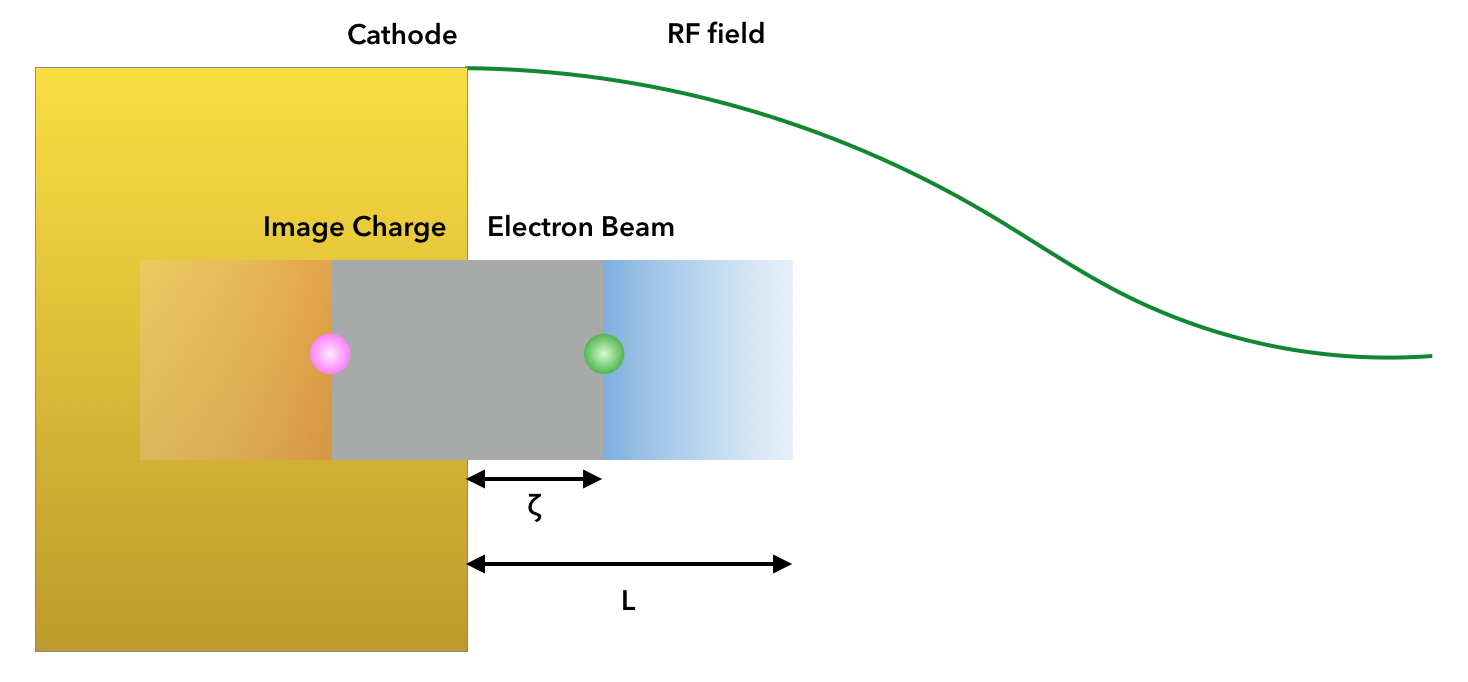
\includegraphics[width=0.9\textwidth]{schottky}
\caption{\label{fig:schottky-mod} 束团中某切片的发射过程示意图}
\end{figure}
如图中所示,在切片 $\zeta$ 从阴极表面出射到离开阴极一定距离的整个过程中,切片 $\zeta$ 以内(纵向相对位置 $< \zeta$)的电荷由于镜像电荷的存在,对切片 $\zeta$ 的作用为零;而切片 $\zeta$ 以外的电荷 $q$ 由于镜像电荷的存在,对切片 $\zeta$ 的作用会加强为两倍。同时考虑引出电场 $E_0$ 以及该切片中电子自身的镜像电荷力,有该切片中电子在发射过程中所感受到的总场强为:
\begin{equation}
-\frac{\partial\phi}{\partial z} = eE_0-e\frac{q}{\varepsilon_0 S}-\frac{e^2}{4\pi\varepsilon_0(2z)^2}
\end{equation}
注意扁平束情形下,空间电荷力对切片 $\zeta$ 的作用力在发射过程中可近似认为不变。上式与标准的单电子发射肖特基模型非常类似,仅需要将标准肖特基模型中的外场 $E_0$ 置换为 $E_0-q/\varepsilon_0S$ 即可,因此切片 $\zeta$ 中电子感受到的有效逸出功为:
\begin{equation}
\phi_{\text{eff}} = \phi_{w} - e\sqrt{\frac{e\big(E_0-(1-\zeta/L)\cdot Q/\varepsilon_0S\big)}{4\pi\varepsilon_0}}
\end{equation}
其中 $Q$ 为束团的总电荷量。各场对逸出功的贡献随切片离开阴极距离 $z$ 的变化如图 \ref{fig:schottky-mod} 所示。
\begin{figure}[htbp]
\centering
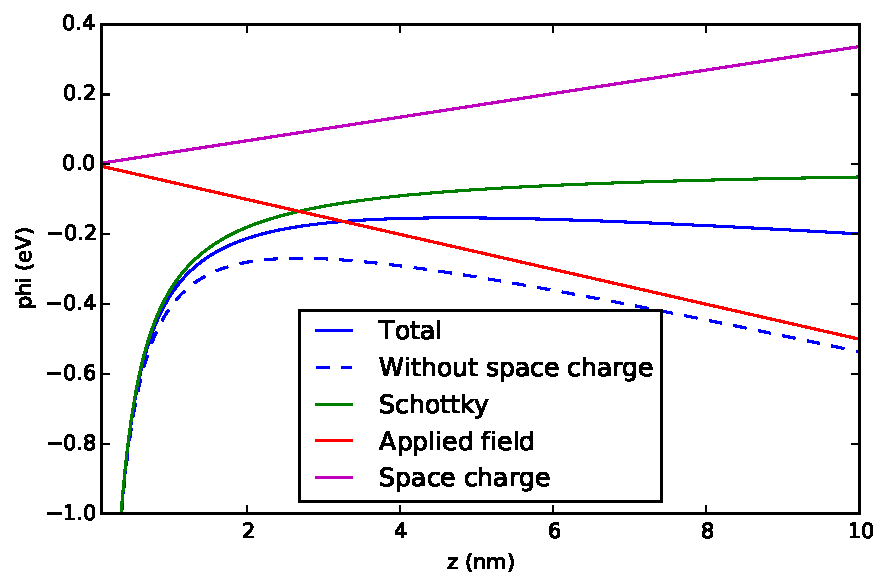
\includegraphics[width=0.6\textwidth]{schottky-mod}
\caption{\label{fig:schottky-mod} 考虑了空间电荷修正的肖特基效应示意图。}
\end{figure}

\subsubsection{考虑了切片发射度差异的束团热发射度}
如第三章所述,计算阴极上热发射度时可忽略动量分布与横向位置间的关系,因此依据统计发射度定义,第 i 个切片的发射度可写做:
\begin{eqnarray*}
\varepsilon_i^2 &=& \sigma_x^2\cdot\langle p_{x,i}^2\rangle \\
&=& \sigma_x^2\cdot\frac{\hbar\omega-\phi_w+e\sqrt{\frac{e\left(E_0-\frac{q_i}{\varepsilon_0 S}\right)}{4\pi\varepsilon_0}}}{3mc^2}
\end{eqnarray*}
这里假定激光纵向均匀分布,因此对于所有切片,其横向 rms 尺寸 $\sigma_{x,i}$ 都相等,等于激光的 $\sigma_{x}$;式中 $q_i$ 为指标大于 i 的切片的电荷量之和。

束团的总发射度为:
\[
\varepsilon^2 = \sigma_x^2\cdot\langle p_{x}^2\rangle
\]
因此有:
\begin{eqnarray}
\varepsilon^2 &=& \sigma_x^2\cdot\frac{\sum\limits_i Q_i\langle p_{x,i}^2\rangle}{\sum\limits_iQ_i} \label{eq:tot-emit-orig}\\
&=& \sigma_x^2\cdot\dfrac{\displaystyle\int_0^{Q}dq\frac{\hbar\omega-\phi_w+e\sqrt{\frac{e\left(E_0-\frac{q}{\varepsilon_0 S}\right)}{4\pi\varepsilon_0}}}{3mc^2}}{\displaystyle\int_0^{Q}dq}\nonumber\\
&=&\sigma_x^2\cdot\frac{\hbar\omega-\phi_w+e\sqrt{\frac{e}{4\pi\varepsilon_0}}\cdot\frac{2}{3}\frac{\varepsilon_0 S}{Q}\left(\sqrt{E_0}^3-\sqrt{E_0-\frac{Q}{\varepsilon_0 S}}^3\right)}{3mc^2}
\label{eq:tot-emit}
\end{eqnarray}
其中 $Q_i$ 为第 i 个切片的电荷量,$Q$ 为总电荷量,$q$ 为切片 $\zeta$ 以内的全部切片电荷量之和。注意上式化求和为积分一步做了变量代换 $Q-q \to q$。

考虑空间电荷限发射($E_0=E_{SC}$)情形,由式 \ref{eq:tot-emit} 可知:
\begin{equation}
\varepsilon = \sigma_x\cdot\sqrt{\frac{\hbar\omega-\phi_w+e\sqrt{\frac{e\cdot\frac{4}{9}E_0}{4\pi\varepsilon_0}}}{3mc^2}}
\end{equation}
也即在空间电荷限发射情形下,发射束团的总发射度相当于不考虑切片空间电荷力时,阴极表面电场强度为 $E_0^*$ 的切片发射度,其中 $E_0^*$ 满足:
\begin{equation}
E_0^*=\frac{4}{9}E_0
\end{equation}
上式启发我们对式 \ref{eq:tot-emit} 进行一定的近似:
\begin{equation}
\varepsilon \approx \sigma_x\cdot\sqrt{\frac{\hbar\omega-\phi_w+e\sqrt{\frac{e\left(E_0-\frac{5}{9}\frac{Q}{\varepsilon_0 S}\right)}{4\pi\varepsilon_0}}}{3mc^2}}
\label{eq:tot-emit-approx}
\end{equation}
近似效果如图 \ref{fig:emit-mod} 所示。

\begin{figure}[htbp]
\centering
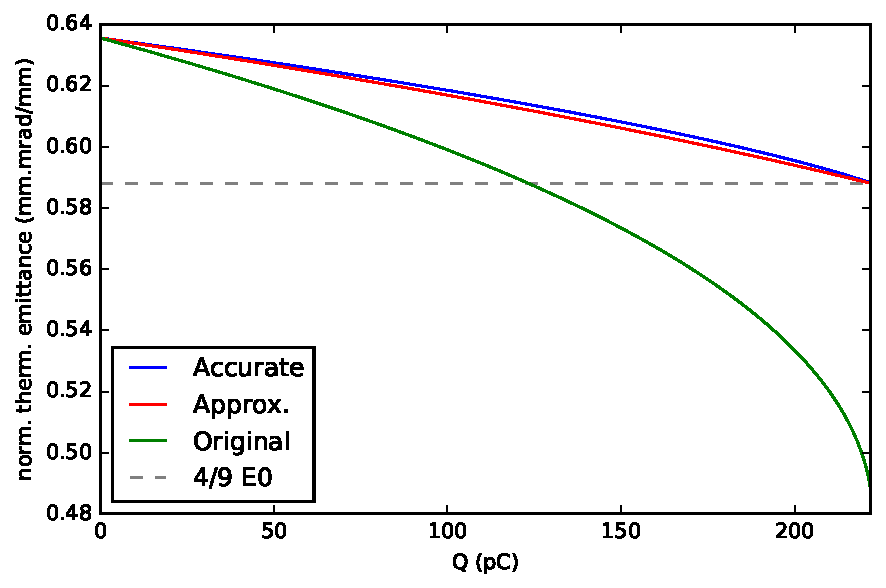
\includegraphics[width=0.6\textwidth]{emit-mod}
\caption{\label{fig:emit-mod} 修正前后的束团归一化发射度随发射电荷量的变化。}
\end{figure}

图 \ref{fig:emit-mod} 给出在 \SI{50}{MV/m} 的引出电场下的铜阴极表面束团热发射度随发射电荷量的变化。图中蓝色曲线对应式 \ref{eq:tot-emit},是精确的束团归一化发射度;红色曲线对应式 \ref{eq:tot-emit-approx},是近似的束团归一化发射度;绿色曲线对应式 \ref{eq:tot-emit-orig},是不考虑切片空间电荷力差异的束团归一化发射度;灰色虚线对应原始束团发射度公式 \ref{eq:tot-emit-none} 中代入 $4/9\cdot E_0$ 的束团归一化发射度。可以看到,精确解和近似解均在空间电荷限发射(对于 \SI{50}{MV/m} 的引出场强,铜阴极的空间电荷限发射对应电荷量约为 222\,pC)情形下收敛到灰色虚线。不考虑束流切片空间电荷力差异的束团发射度则与真实情况差距较大(且始终较真实情况偏小),在空间电荷限发射情形下,相对偏差约 20\%。图 \ref{fig:emit-mod} 还表明,当不考虑空间电荷力时(即发射电荷量为 0),各公式给出的归一化发射度均相等,这也是意料之中的结果。

\subsubsection{扁平束的极限热发射度计算}
上一节我们给出了一个近似效果较好的束团热发射度公式 \ref{eq:tot-emit-approx},下面就利用该式进行扁平束极限热发射度的估计。

依然采用前几节的模型,即激光横向圆均匀分布,纵向均匀分布;阴极材料为铜,光电发射方式为体发射。我们固定阴极表面场强 $E_0$,考察在该场强下阴极的极限热发射度。设激光半径为 $r$,那么 $\sigma_x = r/2$,结合式 \ref{eq:sc-limit},代入式 \ref{eq:tot-emit-approx},有:
\begin{equation}
\varepsilon \ge \frac{r}{2}\cdot\sqrt{\frac{\hbar\omega-\phi_w+e\sqrt{\frac{e\cdot\frac{4}{9}E_0}{4\pi\varepsilon_0}}}{3mc^2}} \ge \frac{1}{2}\cdot\sqrt{\frac{Q}{\varepsilon_0\pi E_0}}\cdot\sqrt{\frac{\hbar\omega-\phi_w+e\sqrt{\frac{e\cdot\frac{4}{9}E_0}{4\pi\varepsilon_0}}}{3mc^2}}
\end{equation}
上式中已不含可变参数(电荷量 $Q$ 是指定的,$E_0$ 也固定),因此扁平束的极限热发射度为:
\begin{equation}
\varepsilon_{\min} = \frac{1}{2\sqrt{3mc^2\varepsilon_0\pi}}\cdot\sqrt{Q}\cdot\sqrt{\frac{\hbar\omega-\phi_w}{E_0}+\frac{1}{3}e\sqrt{\frac{e}{\pi\varepsilon_0}}\cdot\frac{1}{\sqrt{E_0}}}
\label{eq:min-emit-pancake}
\end{equation}
取到极限热发射度的条件为空间电荷限发射($E_{SC}=E_0$)。

\subsubsection{扁平束极限热发射度的讨论}
式 \ref{eq:min-emit-pancake} 给出了扁平束的极限热发射度,观察该式,就得到以下两个基本结论:
\begin{itemize}
\item 极限发射度与发射电荷量 $Q$ 的平方根成正比,即:
\begin{equation}
\varepsilon_{\min} \propto \sqrt{Q}
\end{equation}
\item 若 $\hbar\omega-\phi_w \ge 0$,阴极表面场强越大,极限发射度越小
\end{itemize}
对于铜阴极而言,若采用 266\,nm 激光,则$\hbar\omega-\phi_w = \SI{4.66}{eV}-\SI{4.31}{eV} = \SI{0.35}{eV}$,显然满足第二条,因此想要降低铜阴极的初始热发射度,就必须提高表面场强 $E_0$;同时提高表面场强 $E_0$ 也有助于快速将束流加速到接近光速,抑制低能阶段的空间电荷力对热发射度的破坏。

将场强 $E_0=\SI{50}{MV/m}$,电荷量 $Q=\SI{200}{pC}$ 代入式 \ref{eq:min-emit-pancake},就得到铜阴极在典型条件下的极限热发射度:
\begin{equation}
\varepsilon_{\min, \text{Cu}} = \SI{0.11}{mm\cdot mrad}
\end{equation}
此时对应的激光半径 $r=\SI{379.2}{\mu\meter}$。式 \ref{eq:min-emit-pancake} 可以化成一个对工程更友好的形式:
\begin{equation}
\varepsilon_{\min} = \sqrt{Q}\cdot\sqrt{\frac{5.863(\hbar\omega-\phi_w)}{E_0}+\frac{0.1483}{\sqrt{E_0}}}
\label{eq:min-emit-pancake-eig}
\end{equation}
其中 $\varepsilon_{\min}$ 的单位为 mm$\cdot$mrad,$Q$ 的单位为 nC,$E_0$ 的单位为 MV/m,$\hbar\omega$ 和 $\phi_w$ 的单位为 eV。

上面讨论了 $\hbar\omega-\phi_w \ge 0$ 的情况,$\hbar\omega-\phi_w < 0$ 时情况更加复杂,表面上 $\varepsilon_{\min}$ 不再是 $E_0$ 的单调减函数,而是与 $1/\sqrt{E_0}$ 构成椭圆关系;但由更细致的分析可知,该情形下不可能达到空间电荷限发射条件(因为在空间电荷限达成之前光电子发射就已经由于光电子无法穿过表面势垒而截止了),因而其极限发射度不能再由式 \ref{eq:min-emit-pancake} 描述。具体分析这里就暂不展开了。

\subsection{笔形束的极限热发射度}
笔形束的极限热发射度分析过程与扁平束的非常类似,唯一的不同在于空间电荷限的估算,对于纵横比远大于 1 的笔形束来说,纵向空间电荷场不能再用式 \ref{eq:e-sc-pancake} 来近似。想要给出笔形束中某切片在发射时所感受到的场的(近似)解析表达式较为困难,但如果仅仅想估计笔形束的极限发射度,可以采用如下的想法绕开数学上的困难。

\subsubsection{笔形束的阴极饱和电流}
依然将长束团划分为若干薄切片,考虑某距离阴极为 $z$ 的切片对阴极表面中心的电场,就有(包含镜像电荷效应):
\begin{equation}
E_{SC}(z) = \frac{\sigma}{\varepsilon_0}\left(1-\frac{z}{\sqrt{z^2+r^2}}\right)
\label{eq:slice-sc}
\end{equation}
其中 $r$ 为该切片半径,$\sigma$ 为该切片的面电荷密度。从上面的形式看到,若 $z/r \ll 1$,$E_{SC}(z)\approx \sigma/\varepsilon_0$,即趋向于扁平束中的空间电荷场表达式;若 $z/r \gg 1$,$E_{SC}(z)\approx q/2\pi\varepsilon_0z^2$,其中 $q = \pi r^2 \sigma$ 为该切片电荷量,即趋于点电荷与镜像点电荷对阴极表面的作用。图 \ref{fig:slice-sc} 给出了式 \ref{eq:slice-sc} 中电场随距离 $z$ 的变化。
\begin{figure}[htbp]
\centering
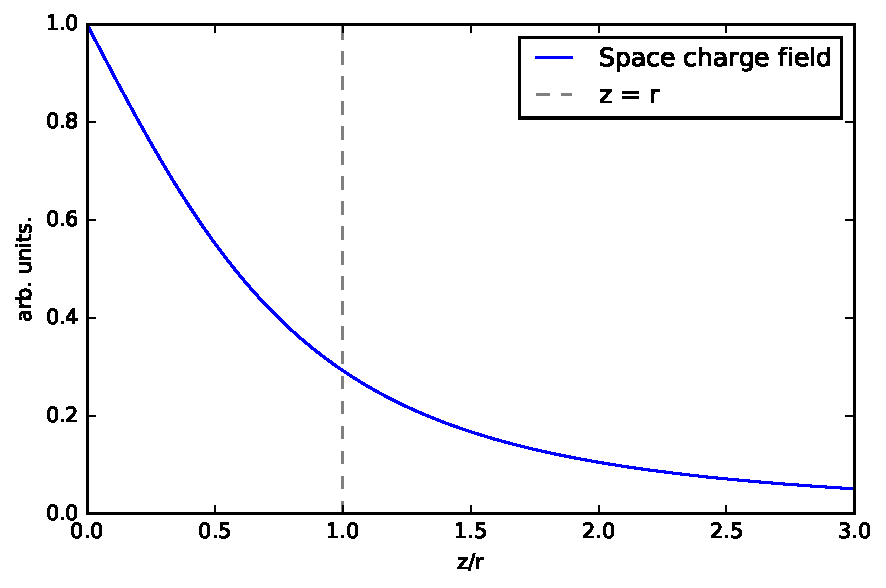
\includegraphics[width=0.6\textwidth]{slice-sc}
\caption{\label{fig:slice-sc} 长束团切片在阴极上的空间电荷场}
\end{figure}
图中可见,当距离 $z$ 与切片半径相等时,该切片对阴极的作用已经相当弱,由此引出了有效作用长度 $z_{\text{eff}}$ 的概念:即只有距离阴极 $z_{\text{eff}}=\eta r$ 以内的切片才会对阴极表面空间电荷场有贡献。将阴极表面有效距离内的束流看做稳定饱和束流(令阴极表面总电场为 0),那么利用 Child-Langmuir 定律,有饱和电流:
\begin{equation}
I_{\text{sat}} = \frac{1}{\sqrt{\eta}}I_0\frac{\sqrt{2}}{9}\left(\frac{eE_0r}{mc^2}\right)^{\frac{3}{2}}
\end{equation}
其中 $I_0=4\pi\varepsilon_0mc^3/e\approx\SI{17}{kA}$ 为 Alfven 电流。模拟证明,在相当大的范围里 $\eta\approx 1$,因此饱和电流可近似为:
\begin{equation}
I_{\text{sat}} \approx I_0\frac{\sqrt{2}}{9}\left(\frac{eE_0r}{mc^2}\right)^{\frac{3}{2}}
\label{eq:sat-I}
\end{equation}

\subsubsection{笔形束的极限热发射度估计}
现在估计笔形束的极限热发射度。由式 \ref{eq:tot-emit-orig} 可知,束团的总发射度为各切片发射度的均方根,而由上节的分析知道,当束团发射长度长于激光横向尺寸时,阴极表面上的空间电荷场强度几乎不再变化;而束团的纵向长度又远远大于横向尺寸,因此束团中绝大多数切片的发射度都相等,等于阴极表面空间电荷场饱和时对应的切片发射度:
\begin{equation}
\varepsilon = \varepsilon_{\text{slice, sat}}
\end{equation}
另一方面,越接近空间电荷限发射,阴极上的饱和空间电荷场越大,那么由有效逸出功修正一节可知,其对应的有效逸出功也就越大,进而饱和切片发射度越小,最小值即阴极表面总电场为 0 时的切片发射度。由此,想达到极限发射度,其条件与扁平束一样,就是空间电荷限发射。注意,为保证空间电荷限发射可达到,这里假定了 $\hbar\omega-\phi_w \ge 0$。

由此,结合饱和电流式 \ref{eq:sat-I},我们有笔形束的极限热发射度估计:
\begin{equation}
\varepsilon \ge \frac{r}{2}\cdot\sqrt{\frac{\hbar\omega-\phi_w}{3mc^2}} \ge \frac{mc^2}{2eE_0}\left(\frac{9Q}{\sqrt{2}I_0\tau}\right)^{\frac{2}{3}}\cdot\sqrt{\frac{\hbar\omega-\phi_w}{3mc^2}}
\end{equation}
其中 $\tau$ 为阴极上的束流脉宽。于是:
\begin{equation}
\varepsilon_{\min} = \left(\frac{9}{16\pi\varepsilon_0}\sqrt{\frac{m}{e}}\right)^{\frac{2}{3}}\cdot\sqrt{\frac{\hbar\omega-\phi_w}{3mc^2}}\cdot\left(\frac{Q}{\tau}\right)^{\frac{2}{3}}\frac{1}{E_0}
\label{eq:min-emit-cigar}
\end{equation}

\subsubsection{笔形束极限热发射度的讨论}
式 \ref{eq:min-emit-cigar} 给出了笔形束的极限热发射度,观察该式,就得到以下两个基本结论:
\begin{itemize}
\item 极限发射度与发射电流 $Q/\tau$ 的三分之二次方成正比,即:
\begin{equation}
\varepsilon_{\min} \propto (Q/\tau)^{\frac{2}{3}}
\end{equation}
\item 极限发射度与阴极表面场强 $E_0$ 成反比,即:
\begin{equation}
\varepsilon_{\min} \propto 1/E_0
\end{equation}
\end{itemize}
第二条结论说明,与扁平束的情况相同,想获得更低的热发射度就要尽可能地提高表面场强。而第一条结论与扁平束的情形相当不同:极限热发射度中出现了阴极上的束流脉宽 $\tau$,这意味着在相同电荷量下,为获得更低的极限热发射度,需要拉长阴极上的束长!

然而阴极表面束流脉宽并不能无限制地拉长,因为过长的束流会占有相当的微波场相位,进而会引入高阶 RF 效应,导致在后续的光阴极枪及注入器中传输时发射度发生不可逆增长。

代入一组典型参数(铜阴极,场强 $E_0=\SI{50}{MV/m}$,电荷量 $Q=\SI{200}{pC}$,激光脉宽 $\tau=\SI{10}{ps}$)到式 \ref{eq:min-emit-cigar},就有此情形下的极限热发射度:
\begin{equation}
\varepsilon_{\min, \text{Cu}} = \SI{0.09}{mm\cdot mrad}
\end{equation}
此时对应的激光半径 $r=\SI{390.4}{\mu\meter}$。式 \ref{eq:min-emit-cigar} 可以化成一个对工程更友好的形式:
\begin{equation}
\varepsilon_{\min} = 1.070\sqrt{\hbar\omega-\phi_w}\cdot\left(\frac{Q}{\tau}\right)^{\frac{2}{3}}\frac{1}{E_0}
\label{eq:min-emit-cigar-eig}
\end{equation}
其中 $\varepsilon_{\min}$ 的单位为 mm$\cdot$mrad,$Q$ 的单位为 pC,$\tau$ 的单位为 ps,$E_0$ 的单位为 MV/m,$\hbar\omega$ 和 $\phi_w$ 的单位为 eV。

\subsection{阴极热发射度与注入器出口处的发射度}
前两节我们讨论了阴极表面的两种发射模式:扁平束发射和笔形束发射。比较二者典型参数下的极限热发射度,可以看到笔形束的热发射度要优于扁平束的热发射度,一些模拟和实验探索也证明将束团初始长度拉长有助于降低光阴极注入器出口处的发射度。然而,阴极上的热发射度与注入器出口处的束流发射度一般并不相等。阴极上产生的束团在后续的传输过程中,会受到束团自身非线性空间电荷力的作用(束团分布只要不是 KV 分布就一定存在非线性空间电荷力);由于束团有一定长度占一定的射频相位,因此射频场的高阶成分也会对束团产生非线性射频场的作用;另外,由于束团具有一定能散,注入器中的各束流操纵元件,例如发射度补偿螺线管线圈,四极磁铁等会对束团产生色散效应。以上各因素都会导致束团初始热发射度有不同程度的增大,因此优化注入器发射度时,不能仅仅将光阴极上的热发射度优化到最小,还要考虑该热发射度是否能够较好地保持到注入器出口,这就要对初始激光参数与注入器各元件的参数进行统一的优化。接下来的章节,先引入双频光阴极微波电子枪的概念,随后应用遗传算法对双频电子枪注入器进行多变量多目标优化,以求达到注入器出口处发射度的较优值。

\section{双频光阴极微波电子枪}
经过多年的模拟和实验探索,目前光阴极注入器出口处的束团横向亮度已经趋近于光阴极表面的最大束流亮度。想进一步提高束流亮度,可以提高阴极表面电场强度,降低光电发射时的电子剩余动能,或者将激光的尺寸从扁平状改变为细长状(笔形束)。光电发射时采用笔形束的基本原理是牺牲光电流的峰值流强,降低空间电荷效应,抑制发射度增长。因此如果采用笔形束方案,为保持光阴极注入器出口处流强足够(一般 FEL 的应用对注入器出口处的流强要求为 30\,A 左右),必须要使用聚束腔(buncher)。然而,由于笔形束的纵向尺寸较大,占有一定的微波相位,RF 发射度就会增长,进而束团的纵向分布在聚束后就会变得高度不对称,这样的束流对于 XFEL 等应用其出光品质就会降低。

为了降低 RF 发射度增长以及减小束团纵向分布不对称性,空间叠加型光阴极电子枪的概念应运而生。典型的空间叠加型光阴极电子枪结构见图 \ref{fig:overlapgun}。

\begin{figure}[htbp]
\centering
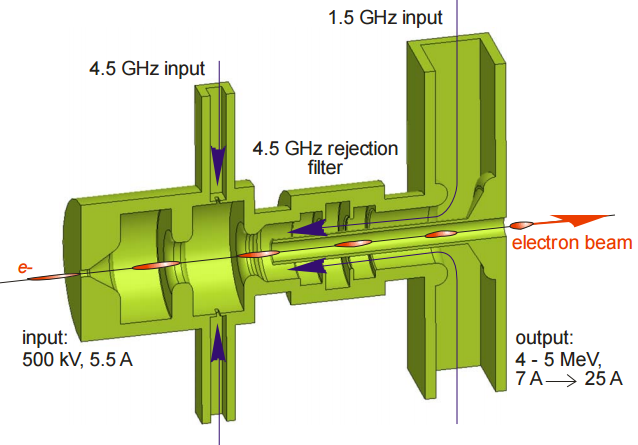
\includegraphics[width=0.6\textwidth]{overlapgun}
\caption{\label{fig:overlapgun} PSI 设计的空间叠加型光阴极电子枪结构图。}
\end{figure}

其原理为:将基模和高阶模(一般是三阶模)叠加在同一个腔体内,那么在某一段 RF 相位区间就会形成一段线性的微波场,如图 \ref{fig:linearfield} 所示。工作时将电子束置于该相位区间,则原来的微波场造成的二阶 RF 效应就被补偿,电子束从始至终处于一个线性场区,其引入的能量调制为线性,从而实现均匀的压缩,即在保持发射度以及峰值流强的情况下,使电子束的纵向分布也尽量均匀,提高后续的出光效率。

\begin{figure}[htbp]
\centering
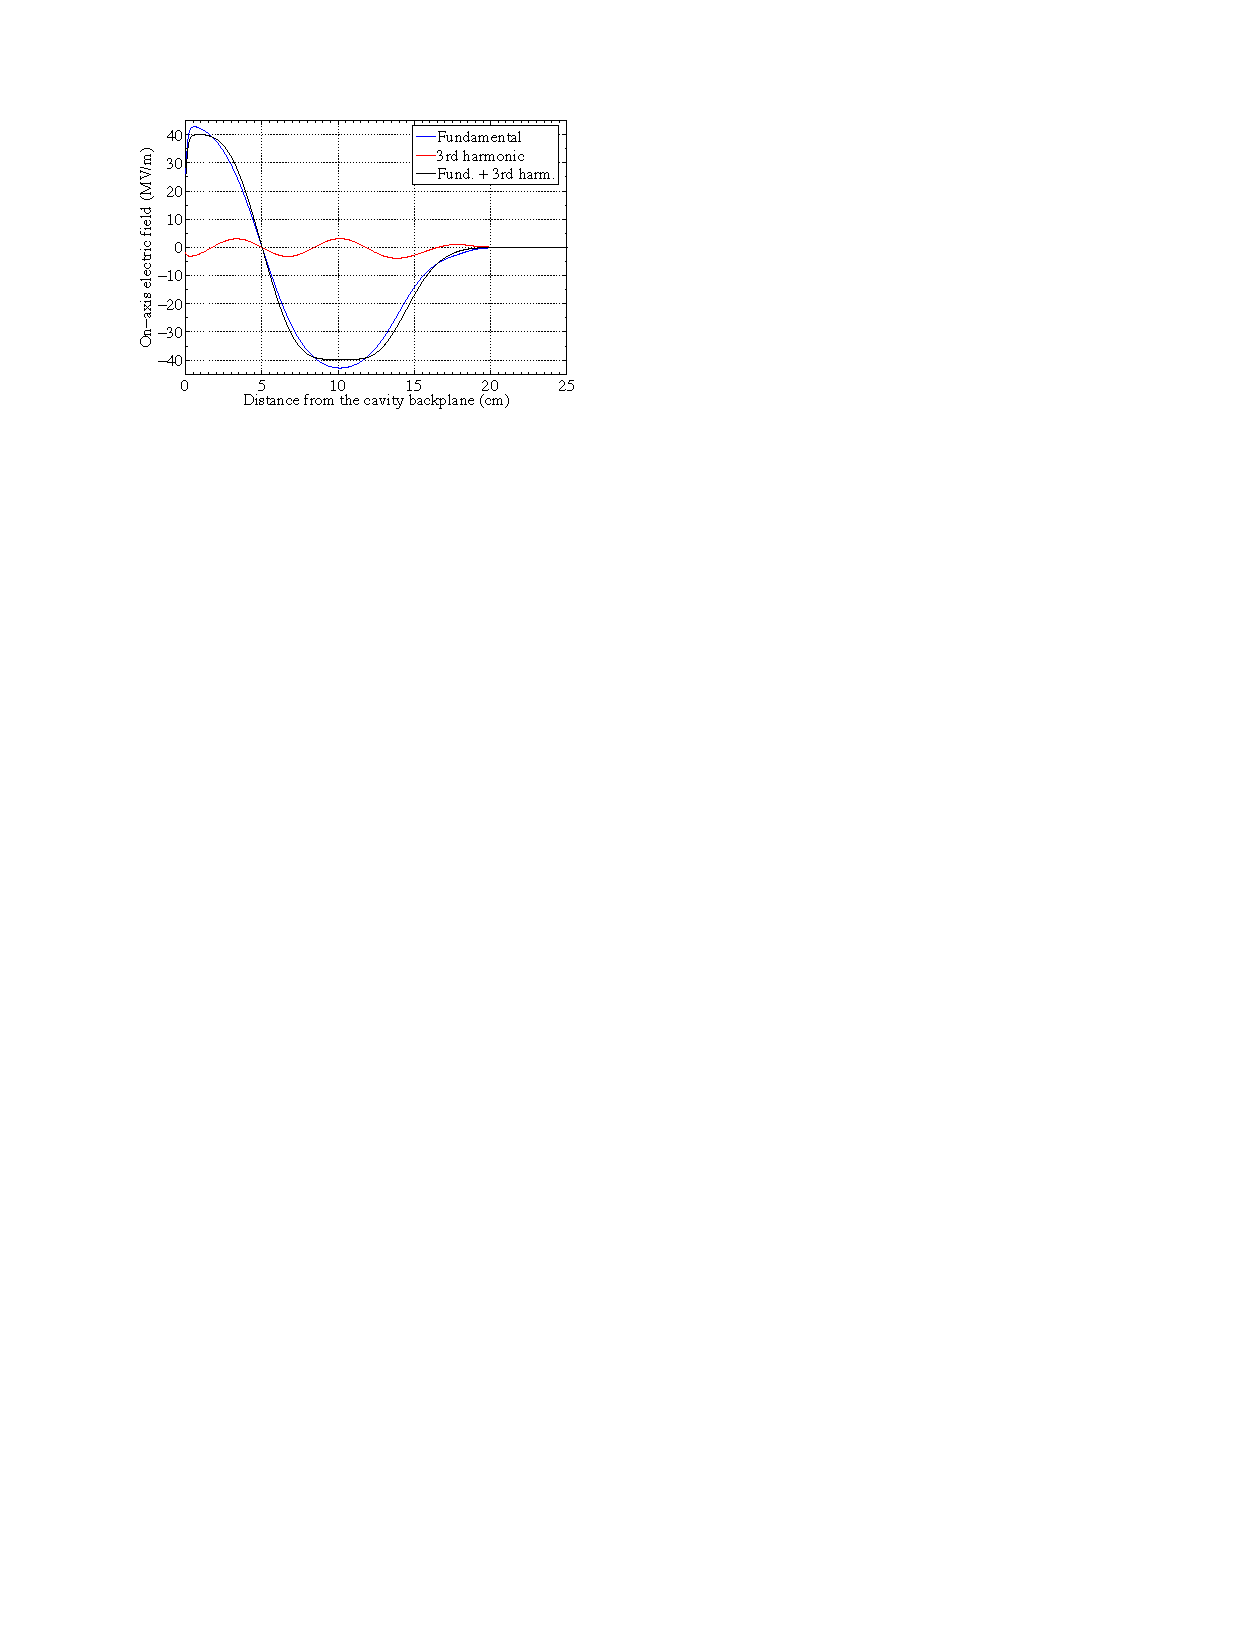
\includegraphics[width=0.6\textwidth]{overlap}
\caption{\label{fig:linearfield} 空间叠加型光阴极电子枪中的微波场。}
\end{figure}

尽管空间叠加型电子枪的原理已经由束流动力学模拟所验证,想真正实现这个想法却是很困难的:一把空间叠加型电子枪需要两个耦合器和一个过滤器,并且要在同一个腔中同时调谐和调平基模和高阶模(HOM)两个模式,其工程难度是巨大的。受此思想启发,我们提出了一种不同的路线来实现双频电子枪,即将两个 RF 模式在空间上分离开,分别将它们放在基模腔和高阶模腔中,并将基模腔和高阶模腔紧凑地组合起来,就形成了空间分离双频电子枪。

实际设计中,我们将一个 BNL 型 1.6 cell S 波段电子枪和一个高阶模腔集成在一起,初始束团的纵向尺寸先被拉长,抑制了空间电荷力发射度的增长,随后在束流经过高阶模腔时进行聚束,这样就可以在注入器出口处获得较高的峰值流强。由于相同的电荷量下,较长束团对应的横向尺寸较小,因此此举也可减小阴极表面初始热发射度。空间分离双频电子枪中的高频腔也同时可对束流纵向相空间进行线性化,从而补偿掉微波场的二阶效应,从而可在注入器出口形成对称束流,这对电子束团的后续应用有很大好处。

\section{空间分离双频电子枪的腔型设计}
我们选择了 S 波段的四阶模 X 波段作为高频腔的工作波段,并利用 Superfish 做电磁场模拟以进行腔结构参数设计。在腔型尺寸设计中,主要考察了以下几个限制条件:1)基频腔和高频腔的工作模式频率要分别为 S 波段和 X 波段;2)S 波段模式的场要调平;3)X 波段模式渗透到 S 波段腔体的场不能太强。为了同时满足三个条件,选定了 S 波段半腔半径,S 波段整腔半径与 X 波段腔半径作为输入变量;两个模式的频率,S 波段模式场平为目标变量,对腔型进行优化。

X 波段模式的场渗透率(X 波段模式在 S 波段腔中最高场强与在 X 波段腔中最高场强之比)可以通过调节 X 波段高频腔的位置进行控制,且后续动力学模拟中可能对高频腔位置有反馈,因此腔型优化可能对于 X 波段高频腔的不同位置反复进行多次。鉴于此,我们借鉴梯度下降法的思想编写了腔型自动优化算法,实现对腔型的自动优化。

\subsection{腔型自动优化算法}
腔型自动优化算法的基本思想如下:假定我们的目标为 $\mathbf{y_t} = (y_{1,t}, y_{2,t}, y_{3,t})^T$,那么优化问题实质是找到使:
\begin{equation}
\label{eq:newton}
\mathbf{y_t} = f(\mathbf{x_t})
\end{equation}
成立的 $\mathbf{x_t}$,其中 $f$ 即系统对输入变量的响应函数,一般情况下具体形式未知(但是对于给定的输入,系统可以给出响应,例如任何一个动力学模拟的模拟结果对于束线的参数的响应函数就是这样的情形)。采用类似牛顿法求根的思想,若我们相信使得式 \ref{eq:newton} 成立的 $\mathbf{x_t}$ 一定存在,那么只要从输入变量初始值 $\mathbf{x} = (x_{1}, x_{2}, x_{3})^T$ 开始,求出该点处响应函数的值 $\mathbf{y} = (y_{1}, y_{2}, y_{3})^T$ 及梯度 $\mathbf{M}$(即雅可比矩阵):
\[
d\mathbf{y} = \mathbf{M}\cdot d\mathbf{x}
\]
及此时的目标差距 $\mathbf{\Delta} = \mathbf{y_t}-\mathbf{y} = (y_{1,t}-y_1, y_{2,t}-y_2, y_{3,t}-y_3)^T$,就可以求出预期的 $\mathbf{x_t^*}$:
\begin{equation}
\label{eq:delta}
\mathbf{x_t^*} = \mathbf{M}^{-1}\cdot\mathbf{\Delta}+\mathbf{x}
\end{equation}
由于一般动力学系统的响应函数并非线性,因此 $\mathbf{x_t^*}$ 一般不会是真解,但若响应函数 $f$ 性质较好,则式 \ref{eq:delta} 会给出一个距离真解更近的解;以该解作为新的输入变量,重复以上步骤,就获得一系列解 $\mathbf{x}, \mathbf{x_t^*}, \mathbf{x_t^{**}, \dots}$ 及对应的目标差距 $\mathbf{\Delta}, \mathbf{\Delta^*}, \mathbf{\Delta^{**}, \dots}$,随着迭代次数增加,解序列会逐渐趋近于真解 $\mathbf{x_t}$,目标差距序列会逐渐趋近于 $\mathbf{0}$。

实际优化中,我们采用下式而非式 \ref{eq:delta} 生成解序列:
\begin{equation}
\label{eq:delta2}
\mathbf{x_t^*} = \eta\mathbf{M}^{-1}\cdot\mathbf{\Delta}+\mathbf{x}
\end{equation}
其中 $\eta$ 为一个 0 到 1 之间的因子,与收敛速度相关。经过实验,我们最终采用 $\eta=1/2$ 进行优化求解。

能够应用以上算法的前提是:1)要保证解存在;2)输入变量与目标变量维数相同(维数可以更高,不限定是三维的)。第二点是保证雅可比矩阵是方阵,有可逆的可能性。因此在腔型优化中,采用了三输入变量,三目标变量的设置。

我们使用 Python 编程实现了上述算法。实现过程的重点是如何给出某点的雅可比矩阵,我们采用了下面的办法:首先计算输入变量 $\mathbf{x}$ 对应的输出 $\mathbf{y}$;随后对于输入变量的某一分量 $x_i$ 取增量 $dx_i$ 变为 $x_i^{\prime}$,计算输入变量为 $\mathbf{x}_i^{\prime} = (x_1, x_2,\dots,x_i^{\prime},\dots,x_n)^T$ 的响应 $\mathbf{y}_i^{\prime}$,也即仅将输入变量第 i 维取增量时的系统响应,那么雅可比矩阵就可写为:
\begin{equation}
\label{eq:jacob}
\mathbf{M} = \left(\frac{\mathbf{y}_1^{\prime}-\mathbf{y}}{dx_1}, \frac{\mathbf{y}_2^{\prime}-\mathbf{y}}{dx_2}, \dots, \frac{\mathbf{y}_n^{\prime}-\mathbf{y}}{dx_n}\right)
\end{equation}
对于本节中的腔型优化问题,可以估算迭代一次所需的模拟次数:对原始输入变量求输出需要一次模拟,生成雅可比矩阵需要三次模拟,因此一次迭代需要四次模拟。实际优化中,发现该优化算法的收敛速度极快,对于较好的初始输入值,达到精度要求或收敛(由于加工精度有限,模拟中各尺寸的精度到 10\,$\mu$m 量级,因此迭代进行到一定次数后新给出的输入变量由于四舍五入而保持与上一组输入变量相同,此时优化算法收敛,但给定的目标变量精度要求可能并未达到)只需要三次左右的迭代,因此一次完整优化只需要运行 12 次模拟,效率很高。

\subsection{腔型优化后的结构参数及场分布}
我们将 X 波段高频腔放在离 S 波段腔尽可能近(但保持场渗透率低于千分之一)的位置,应用自动优化算法,最终得到整体双频电子枪腔型及场分布见图 \ref{fig:field_sx}。S 波段腔型微波及结构参数见表 \ref{tab:geo_s},X 波段腔型微波及结构参数见表 \ref{tab:geo_x}。
\begin{figure}[htbp]
	\centering
	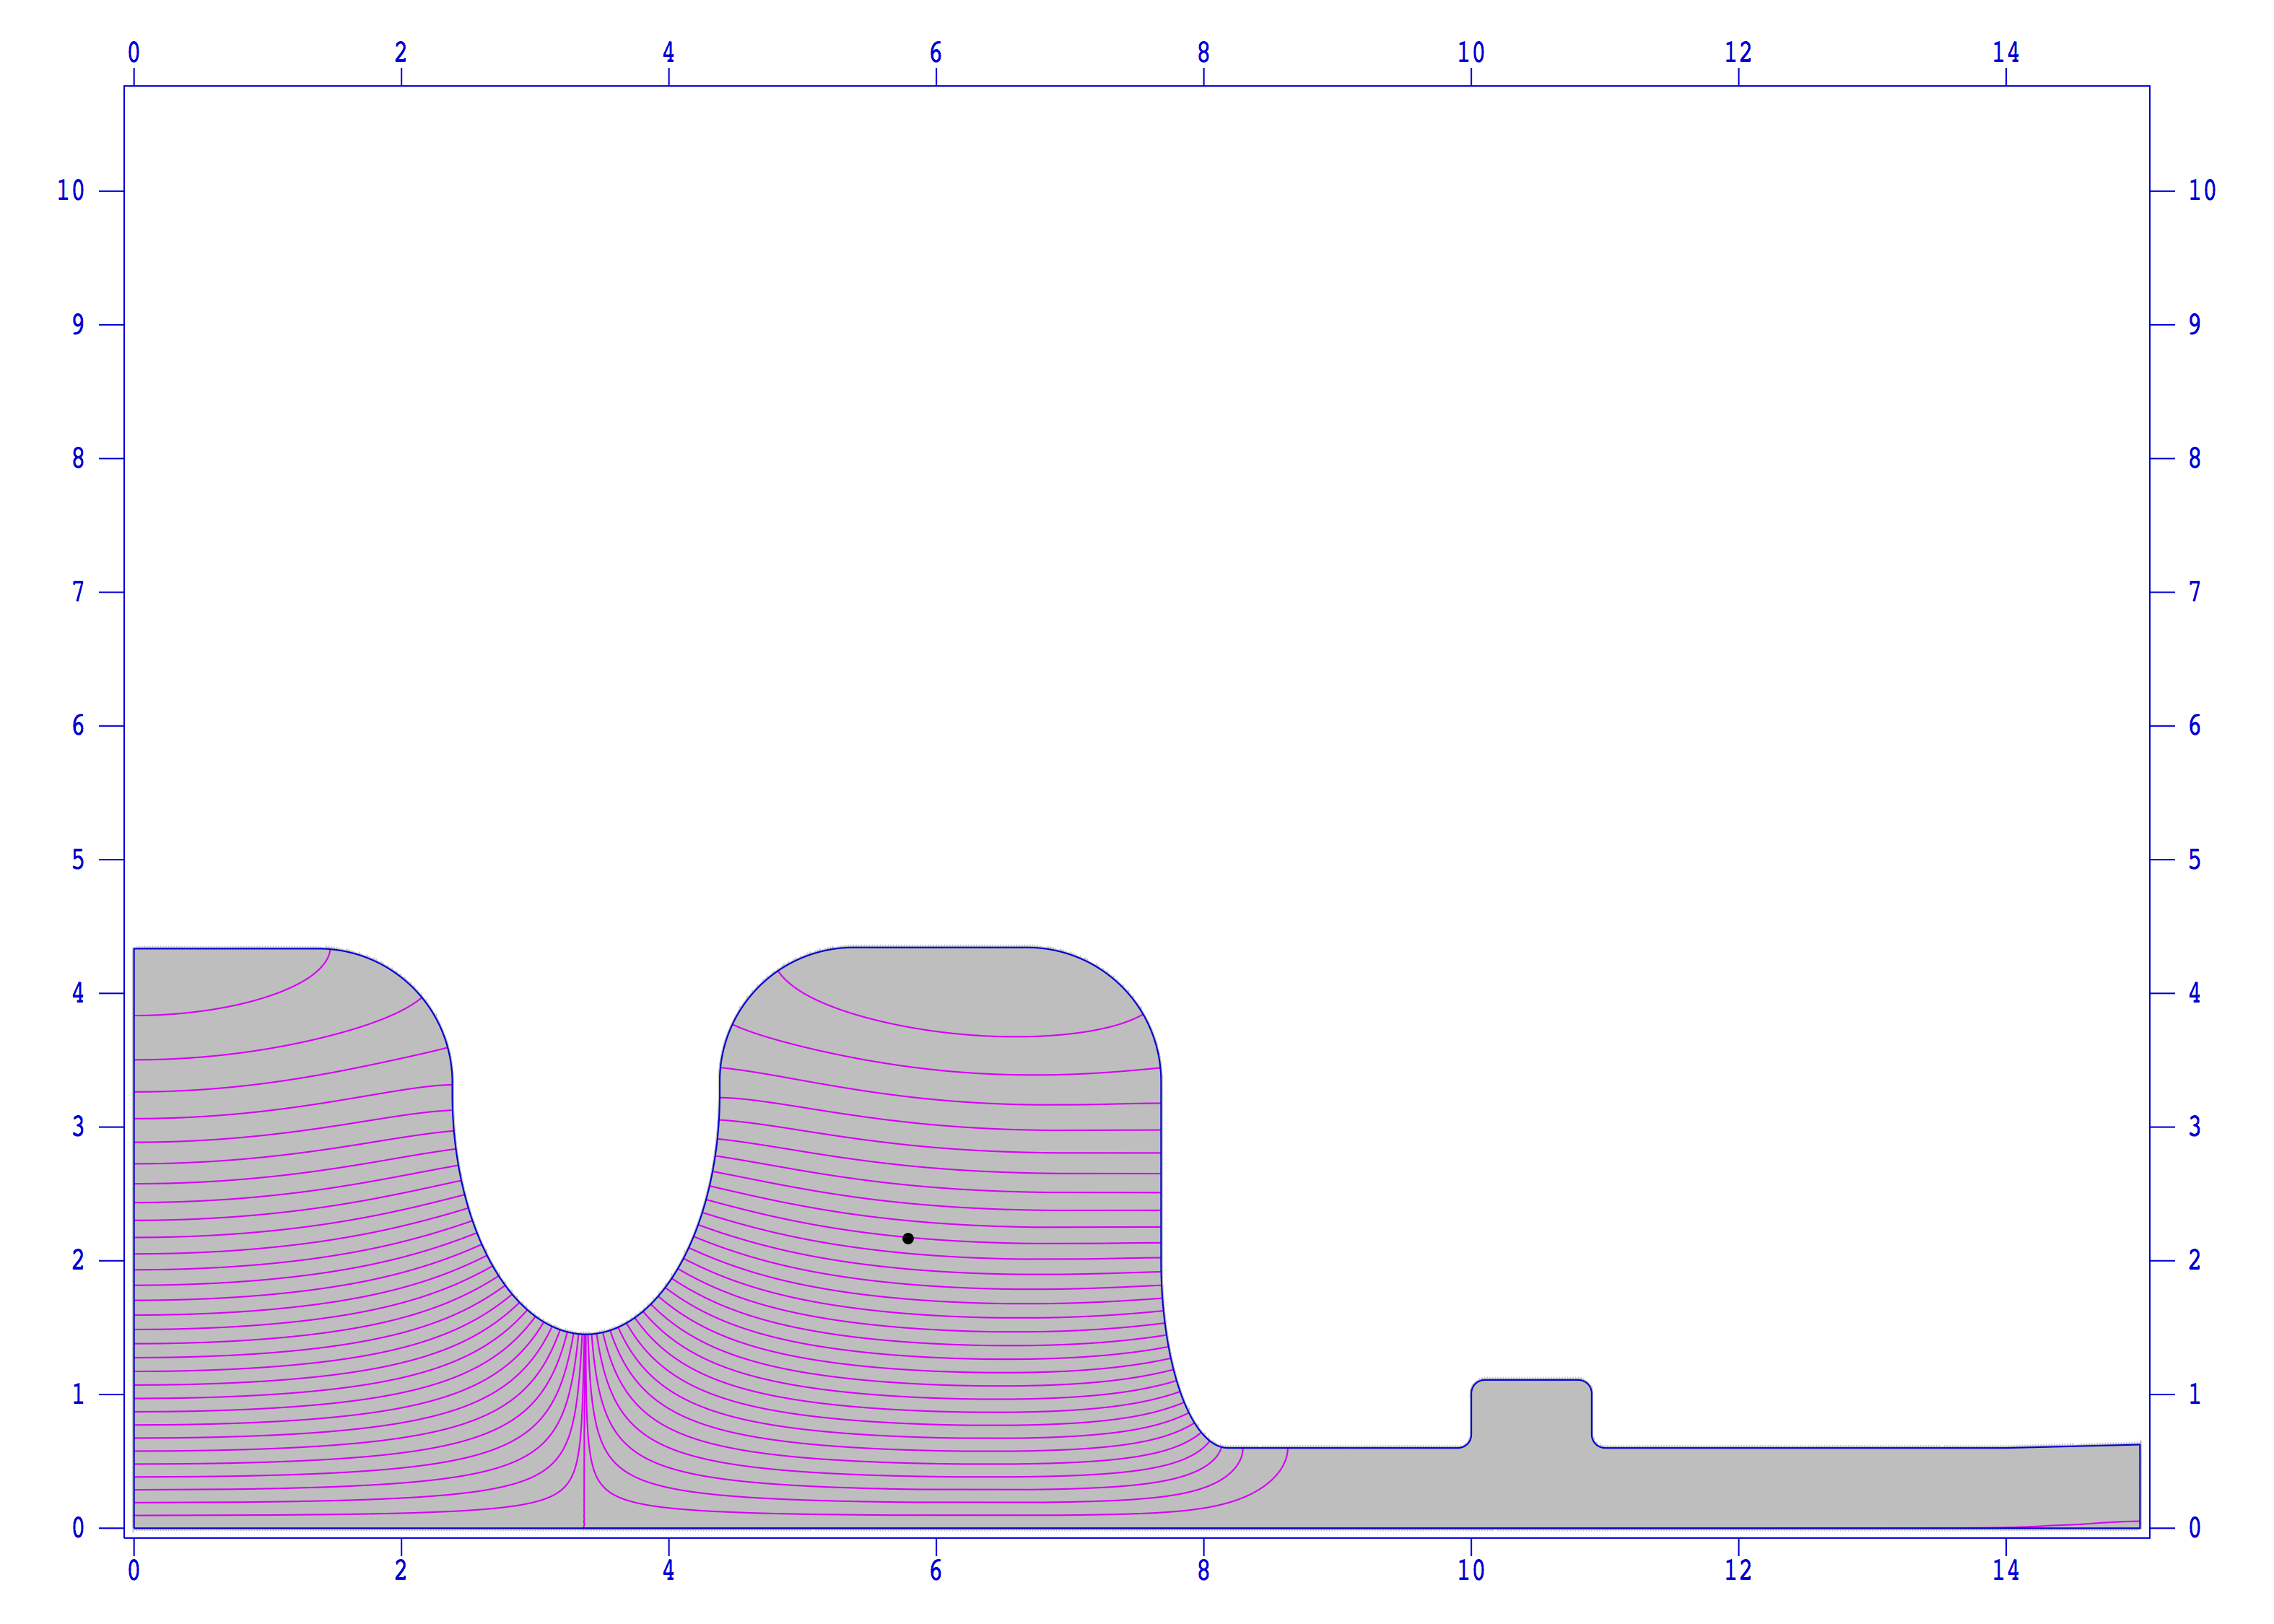
\includegraphics[width=0.45\textwidth]{field_s}
	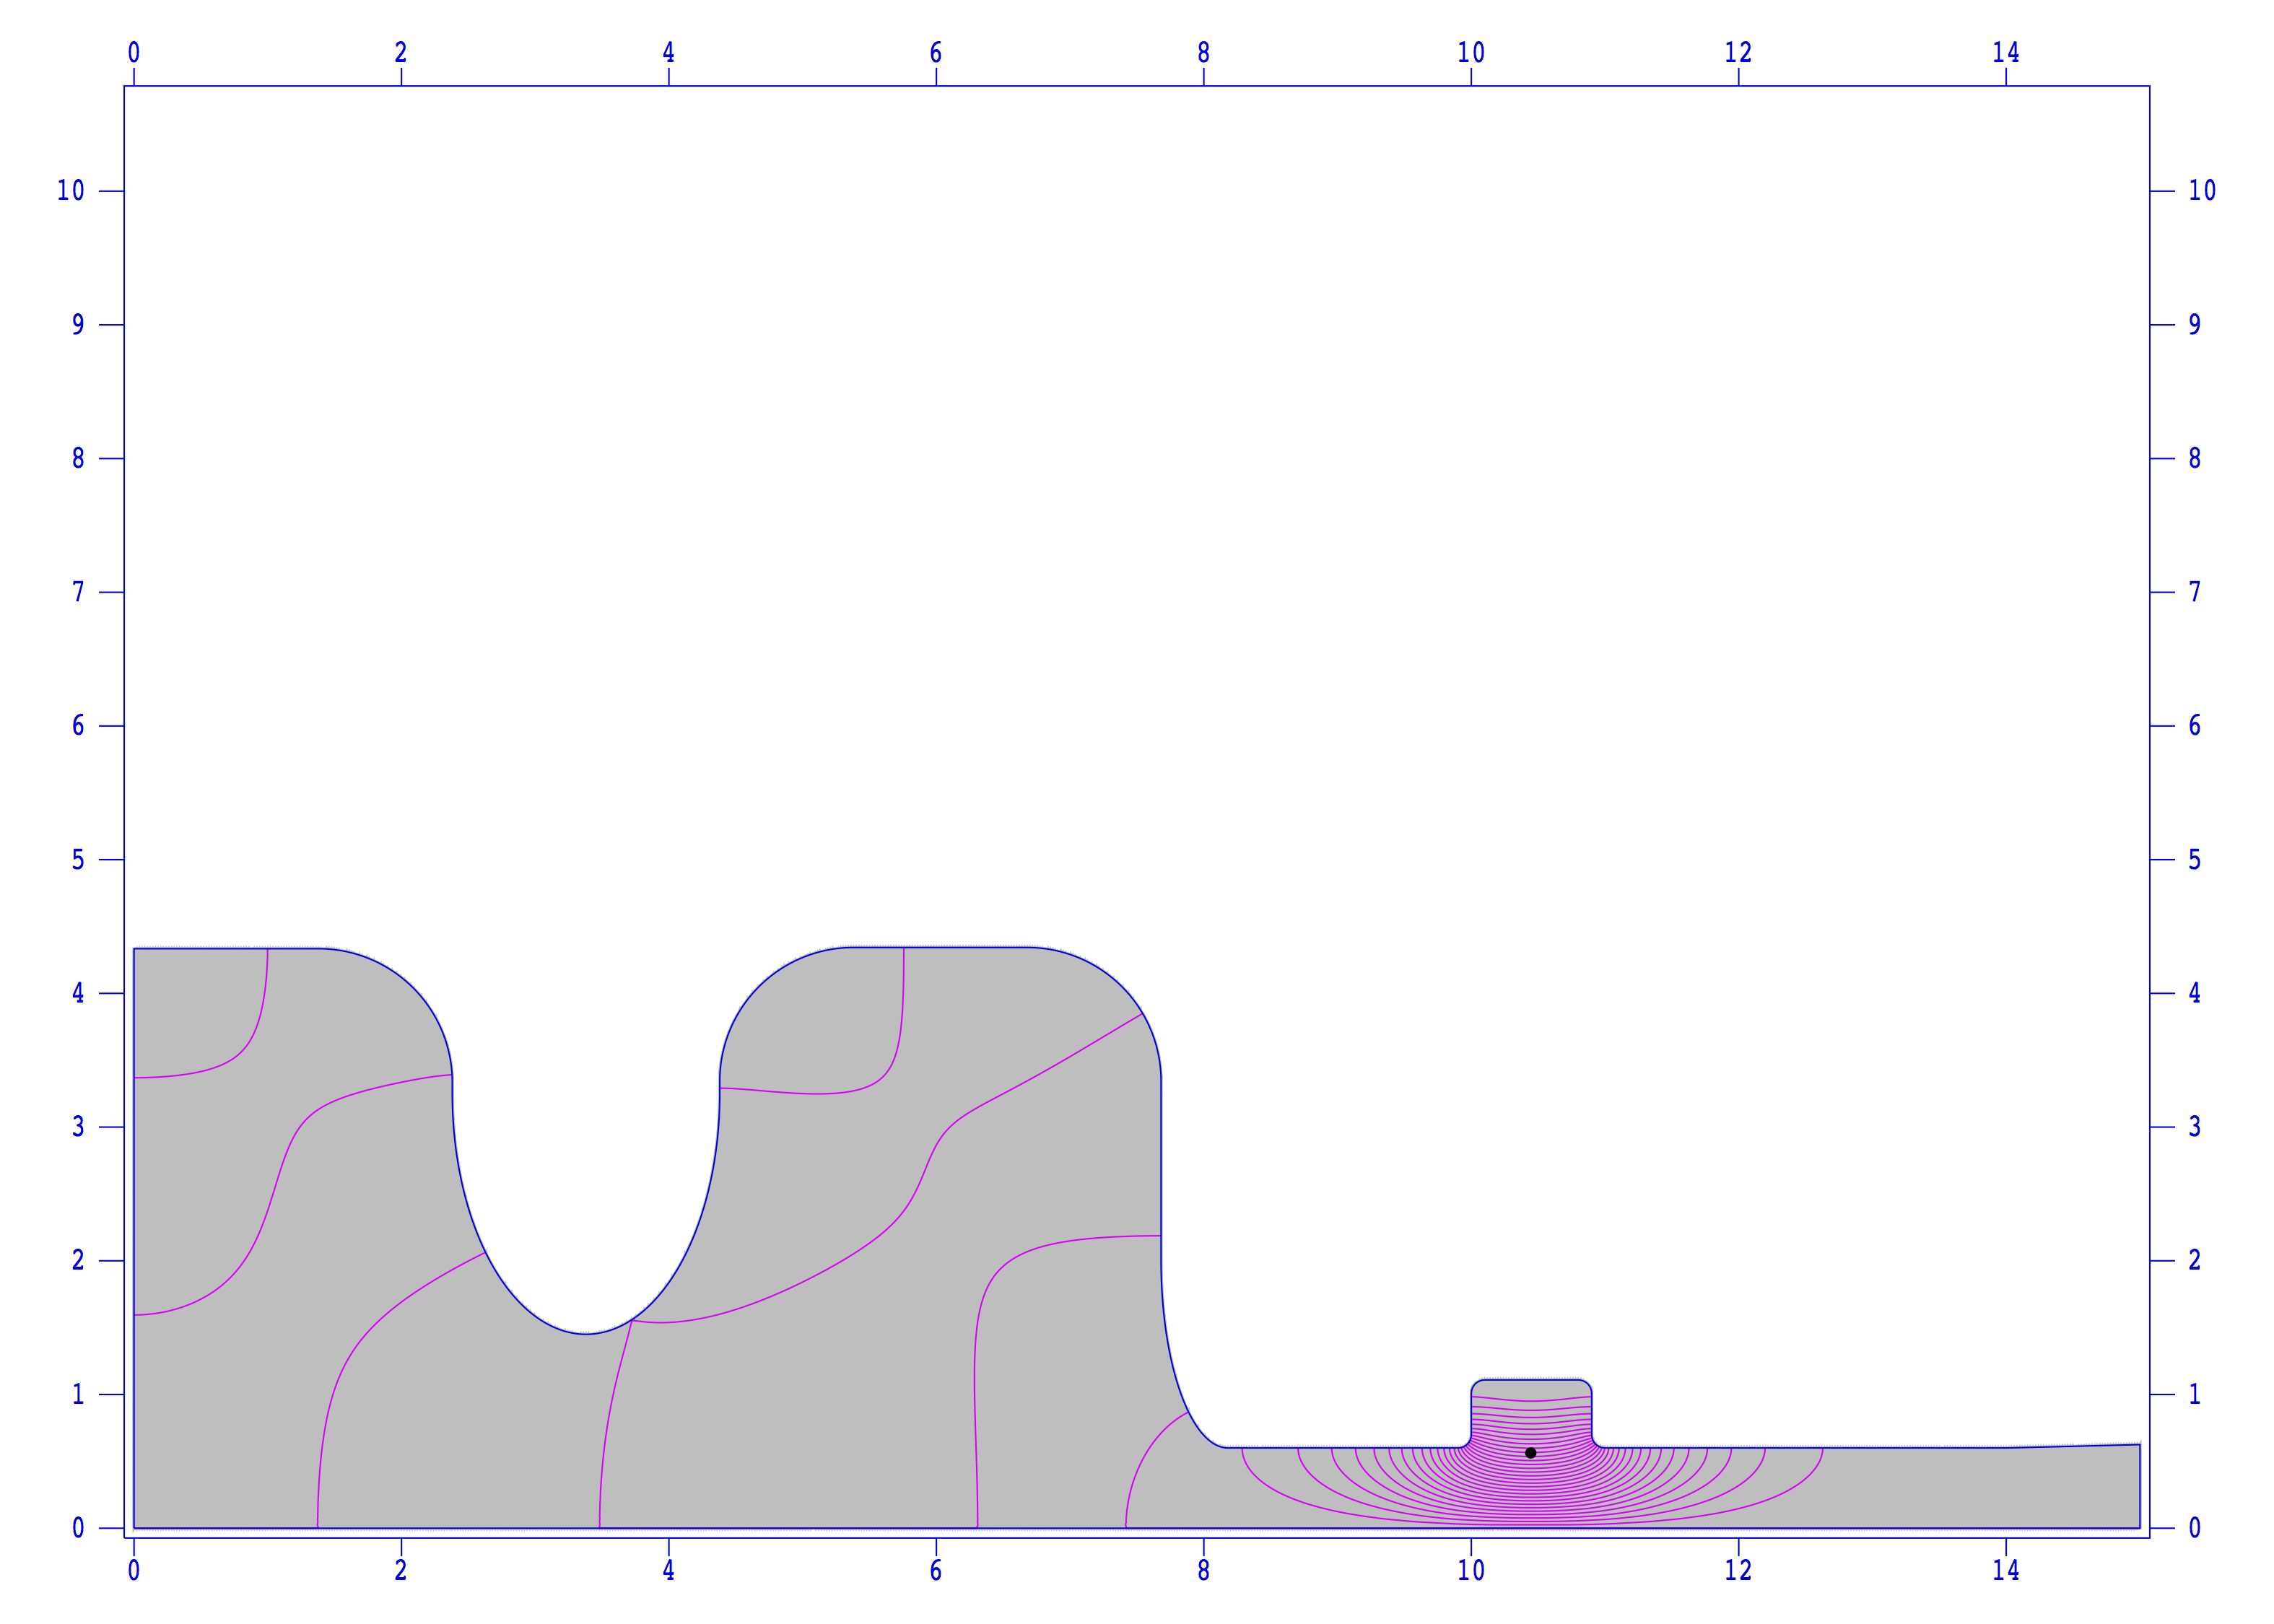
\includegraphics[width=0.45\textwidth]{field_x}
	\caption{
	双频电子枪中的电场分布。左图:S 波段基模电场分布;右图:X 波段高阶模电场分布。}
	\label{fig:field_sx}
\end{figure}

\begin{table}[htbp]
\centering
\caption{\label{tab:geo_s}
S 波段腔结构参数。}
\begin{tabular}{lll}
\toprule
参数 & 值 & 描述\\
\midrule
freq & \SI{2856.00}{MHz} & 微波频率  \\
flatness & 0.9996 & 场平  \\
\midrule
$l_h$ & \SI{3.38}{cm} & 半腔长度  \\
$r_h$ & \SI{4.3341}{cm} & 半腔半径  \\
$c_h$ & \SI{1}{cm} & 半腔倒角半径  \\
$j_h$ & \SI{1}{cm}, \SI{1.8}{cm} & 半腔盘片长、短轴 a、b \\
$l_f$ & \SI{4.8}{cm} & 整腔长度  \\
$r_f$ & \SI{4.3431}{cm} & 整腔半径  \\
$c_f$ & \SI{1}{cm} & 整腔倒角半径  \\
$j_{f, l}$ & \SI{1}{cm}, \SI{1.8}{cm} & 整腔左盘片长、短轴 a、b \\
$j_{f, r}$ & \SI{0.5}{cm}, \SI{1.4}{cm} & 整腔右盘片长、短轴 a、b \\
$r_{f, t}$ & \SI{1.45}{cm} & 束流管道半径  \\
\bottomrule
\end{tabular}
\end{table}

\begin{table}[htbp]
\centering
\caption{\label{tab:geo_x}
X 波段腔结构参数。}
\begin{tabular}{lll}
\toprule
参数 & 值 & 描述\\
\midrule
freq & \SI{11424.25}{MHz} & 微波频率  \\
penetration & $3.02\times10^{-4}$ & 场渗透率  \\
\midrule
$p$ & \SI{9.9}{cm} & 腔起始位置  \\
$l$ & \SI{1.1}{cm} & 腔长度  \\
$r$ & \SI{1.1088}{cm} & 腔半径  \\
$c$ & \SI{0.1}{cm} & 腔倒角半径  \\
$j$ & \SI{0.1}{cm} & 腔盘片半径  \\
$r_t$ & \SI{0.6}{cm} & 束流管道半径  \\
\bottomrule
\end{tabular}
\end{table}

\begin{figure}[htbp]
	\centering
	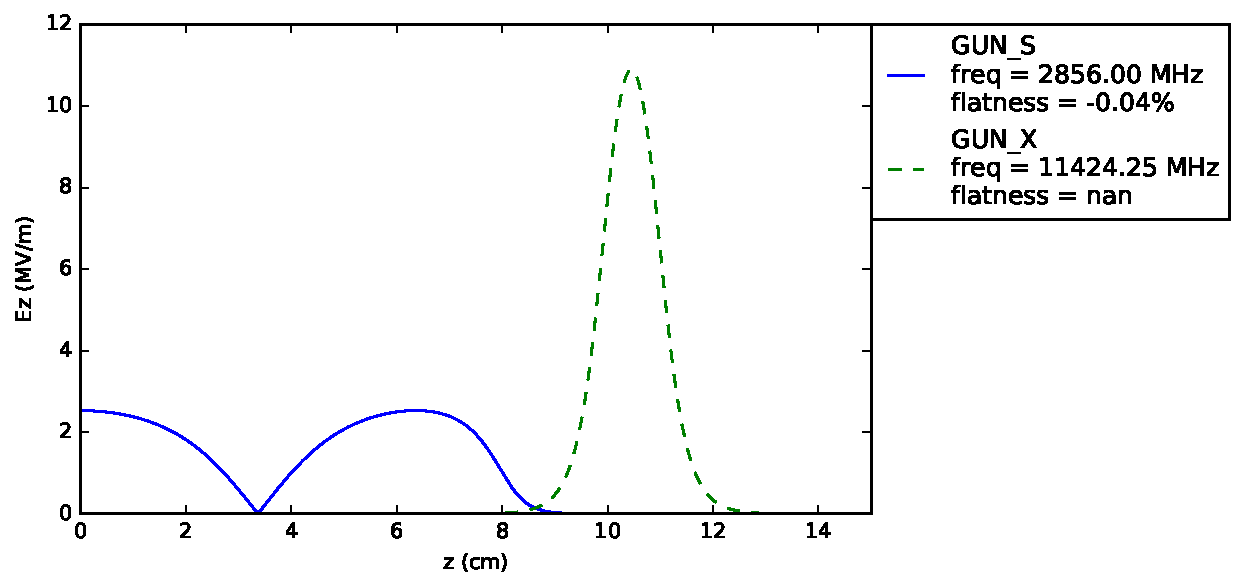
\includegraphics[width=0.8\textwidth]{sx-dist}
	\caption{
	S/X 双频电子枪中的轴线电场分布。注意纵座标并不代表实际场强,而是分别对 S 波段和 X 波段腔中模式能量进行归一化后的场强。}
	\label{fig:sx-fielddist}
\end{figure}
S/X 双频电子枪的轴线场分布见图 \ref{fig:sx-fielddist}。从图中可见,S 波段半腔和整腔中的场强基本平整,X 波段高阶模几乎没有渗透进 S 波段腔体中,自动优化算法较为可靠。另外也可看到,由于 X 波段腔的存在,S 波段整腔中场强分布变得稍稍不对称,这个不对称性对动力学的影响有待后续模拟研究。

\section{空间分离双频电子枪的动力学验证}
腔型设计好后,需要对双频电子枪的性能进行验证,我们利用 Astra 来做空间分离双频电子枪的动力学模拟。人们真正关心的是注入器出口处束流的参数而非仅仅电子枪出口处的束流参数,因此双频电子枪被放入一个类 LCLS 的光阴极注入器(见图 \ref{fig:injector-x})中进行动力学优化。为验证双频电子枪的亮度提升的效果,需要与普通电子枪的注入器优化结果进行比对。

我们关心的物理量为注入器出口处束流的峰值流强和发射度(100\% 投影发射度,95\% 投影发射度及切片发射度),在束团电荷量一定的情况下(200\,pC),注入器出口处峰值流强可以近似认为只由束团长度决定,因此最终的目标变量设置为注入器出口处束流的 rms 长度与投影发射度。如图 \ref{fig:injector-x} 中所示,整个注入器由双频电子枪,螺线管线圈及两段加速管构成,可优化的变量为:
\begin{itemize}
\item {\sf 激光}:激光长度及横向尺寸
\item {\sf 双频电子枪}:S 波段腔的场强和相位;X 波段腔的场强和相位
\item {\sf 螺线管线圈}:位置和强度
\item {\sf 加速管}:第一段加速管位置和场强;第二段加速管位置和场强
\end{itemize}
其中 S 波段腔的场强应该取可取的最大值,因为阴极表面场越强对空间电荷发射度增长的抑制效果就越好;第二段加速管一般紧贴第一段加速管,因此只要第一段加速管位置确定,第二段的位置也随之确定,不需要优化。从上面的分析看,完整的注入器需要优化 10 个变量,若采用人工方式优化不仅工作量/耗时巨大而且无法保证取到全局最优解。鉴于此,我们采用了遗传算法(Genetic Algorithm,GA)对该多变量问题进行优化。
\begin{figure}[htbp]
	\centering
	
\includegraphics[width=0.9\textwidth]{injector-x}	
	\caption{S/X 双频电子枪的注入器布局示意图。}
	\label{fig:injector-x}
\end{figure}

\subsection{遗传算法优化器}
\subsubsection{NSGA-II}
我们采用了经典而高效的算法 NSGA-II(Nondominated Sorting Genetic Algorithm II)来驱动遗传算法优化器。
\begin{figure}[htbp]
	\centering
	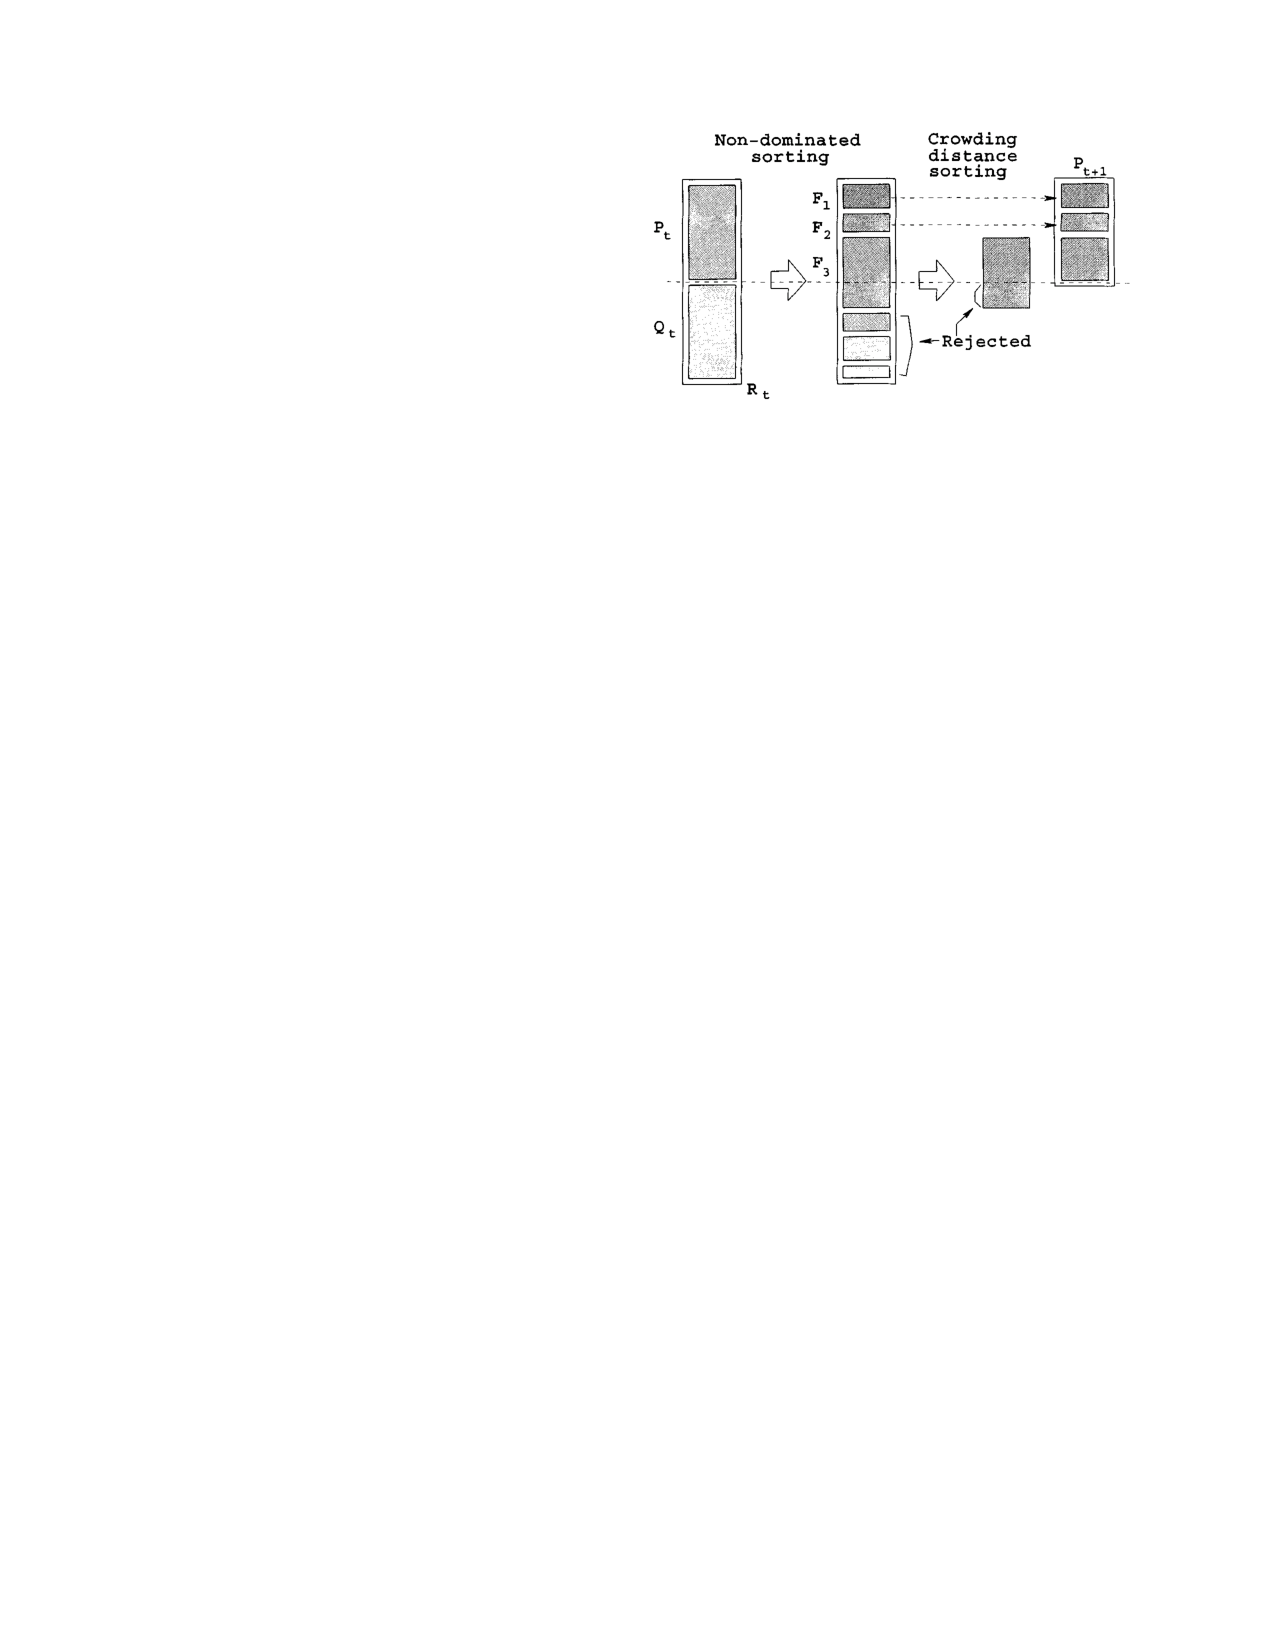
\includegraphics[width=0.6\textwidth]{nsgaii}	
	\caption{NSGA-II 算法原理示意图。}
	\label{fig:nsgaii}
\end{figure}
NSGA-II 的基本原理如图 \ref{fig:nsgaii} 所示,NSGA-II 在进化过程中,同时保留父代和子代,将相邻两代按照种群距离进行筛选,并分为一等公民,二等公民等;产生新的子代时,先从一等公民中按性状优良程度挑选,再依法炮制挑选二等公民,直至达到种群容量上限;新挑选出的子代再分成两组进行 crossover。上述过程一直进行下去,直至种群收敛,此时算法将给出一组最优解,即 Pareto 前沿。多次改变初始种群进行 NSGA-II,就可以获得全局最优解集。

\subsubsection{遗传算法优化器的逻辑结构}
遗传算法优化器逻辑上分为四部分:生成器,运行器,后处理器以及迭代器。下面首先介绍优化器的运行方式,再分别介绍四部分各自的用途。

优化器需要一个已经运行通过的模拟算例作为起始算例,该模拟算例一般体现为一个文件夹,其中包含模拟的输入文件,以及模拟所需要的场分布等附加文件。优化器运行时,对初始算例中的输入文件进行解析,给出输入文件中所有重要的可变参数,随后根据优化器配置文件中设置的具体关心的参数以及各参数的可变范围,依据初始算例,对其参数进行覆盖,随机生成给定容量的初始种群。随后优化器调用动力学模拟程序(例如 Astra)对初始种群的每个个体进行模拟,模拟结束后对模拟结果进行后处理,最后该种群的后处理结果经过汇总分析后,产生新一代种群,依此类推,直到达到优化目标或超出预设资源(时间/存储空间等),优化结束。

\red{这里要插一张流程图。}

在上面的过程中,生成器会根据迭代器提供的输入参数,基于初始算例给出新的待模拟算例;运行器负责调用动力学模拟软件对生成器给出的待模拟算例进行模拟;后处理器接受运行器模拟完成的算例,并对模拟结果进行统计,得到关心的参数(例如注入器出口处束长,发射度等);迭代器则扮演了优化过程的大脑的角色,它根据后处理器给出各算例的参数,给出下一组待模拟算例的输入参数(例如激光尺寸,腔的相位、强度等),同时迭代器还承担着控制整个优化进程的任务,也即它需要根据情况判断是否优化条件达成,是否超时/超储存空间而中止优化等。

以上是遗传算法优化器的一般逻辑结构,该结构并不仅限于遗传算法优化,而是适用于几乎一切加速器中的束流动力学模拟优化任务。在处理不同任务时,只需要根据优化目标和优化方法对迭代器进行定制即可。例如,要对束线中某个参数进行扫描,那么迭代器的逻辑就是根据待扫描参数的上一个取值,给出待扫描参数的下一个取值;对于支持并行计算的平台,实现可以更加简单和快速:迭代器初始化时直接给出待扫描参数全部可能取值,那么该扫描任务一次迭代就完成了。对于本章所采用的遗传算法而言,迭代器执行遗传算法的筛选过程,将父代中符合要求的个体留下,crossover/变异后产生下一代种群。

上面描述的优化器逻辑结构也自动具有扩展功能:例如运行器可以支持调用各种模拟软件,如 Astra,GPT,Parmela 等,只需要为相应的模拟软件写好调用接口即可;而迭代器的具体实现也可以多种多样,甚至可以由人来担任迭代器,根据后处理器给出的上一代性能,决定下一代的优化方向。

\subsubsection{遗传算法优化器的编程实现}
我们采用 Python 编程实现了遗传算法优化器的逻辑结构。优化器程序分为以下六个文件:
\begin{itemize}
\item {\sf astracore.py}:生成器与运行器,负责读取初始模拟算例,接受输入参数生成新算例以及调用 Astra 程序进行模拟计算
\item {\sf plotplugins.py}:后处理器的图形部分,负责对模拟结果进行可视化,例如画出横/纵向相空间,束团纵向密度分布等
\item {\sf statplugins.py}:后处理器的统计部分,负责对模拟结果进行统计,给出发射度/能散/束长/切片发射度等参数
\item {\sf physicshelper.py}:基础的物理运算助手,进行如波长/能量转换,时间/长度转换及 $\beta$/$\gamma$ 等相对论因子转换等常见运算
\item {\sf gaoptimizer.py}:迭代器的引擎,实现了 NSGA-II 算法
\item {\sf main.py}:优化器入口,迭代器的流程控制逻辑,负责产生初始种群,利用 NSGA-II 引擎进化种群,并在满足一定条件后中止进化并产生断点;支持从断点处继续进化的功能
\end{itemize}
遗传算法优化器的核心文件是 {\sf gaoptimizer.py},其内部采用了 DEAP 库作为遗传算法支持库,采用 SCOOP 库实现多核并行计算。有了并行计算的支持,遗传算法优化器才有应用的可能。{\sf main.py} 是遗传算法优化器的入口,其中配置了束线信息,输入变量,优化目标以及遗传算法参数等信息,要应用遗传算法优化器进行束线优化,只需要修改 {\sf main.py} 文件即可。

\subsubsection{遗传算法优化器的运行流程}
遗传算法优化器需要运行在支持并行运算的大型机上。假设占用大型机的 N 个处理器核,其中一个核为主核,其它核为附属核(worker)。一次优化开始时,优化器向主核提交任务,主核调用迭代器产生容量为 N 的初始种群,并调用生成器产生全部模拟算例;随后将每个算例分配到不同的核上,调用运行器进行模拟;所有核上的模拟并行进行,各核之间在模拟过程中无数据交换。注入器在不同输入参数下模拟时间会有伸缩(例如某些电子枪相位可能导致束团反轰,模拟会提前结束),而下一代种群的基因产生需要等上一代模拟彻底结束后才能开始,因此种群的模拟时间等于该种群中耗时最长的个体所用的模拟时间。当种群中全部个体均模拟完毕,各核将模拟结果返回给主核,主核调用后处理器对模拟结果进行后处理(一般是统计注入器出口处 rms 束流长度核 100\% 投影发射度),并将各算例的数据处理结果汇总,调用迭代器根据 NSGA-II 的规则进行筛选、crossover 以及变异,产生下一代种群。循环上面步骤,直到满足跳出条件或达到优化目标,就完成一次遗传算法优化。

遗传算法优化器在每一代种群模拟结束后,都会将该代种群的后处理结果写入一个名为 {\sf ghist} 的文件中,因此即使优化突然中断,{\sf ghist} 文件也保存了从初代种群到中断前种群的全部历史;再次启动优化时,优化器会首先尝试读取 {\sf ghist} 文件,并以最近的一代种群作为起点,继续进化。这就是从断点继续进化的实现原理。

\subsection{遗传算法优化平台}
为保证优化时间在可接受的范围内,我们采用了清华大学探索 100 高性能计算平台作为遗传算法优化器的运行平台。探索 100 高性能平台共有 740 个计算节点,8800 个处理器核。处理器核按照刀片(board)组织,一个刀片上有 12 颗处理器核,一个刀片对应一个计算节点;刀片按照刀片箱(cabinet)放置,每个刀片箱有 20 个刀片,共有 37 个刀片箱。因此定位某计算节点时,采用 c[xx]b[yy] 的方式,其中 [xx] 和 [yy] 为数字,例如 c01b02 就是第一个刀片箱的第二块刀片对应的计算节点。

对于遗传算法驱动的双频电子枪注入器动力学优化,一般选取种群容量是 12 的整数倍(这样就可以占用若干完整的刀片进行并行计算,由于同一个刀片上各核间的数据传输速度远高于不同刀片核间的数据传输速度,占用完整的刀片可使模拟数据的传输更快),为保证 Pareto 前沿的覆盖性,种群容量不能太小,因此常用 120、240 以及 360 的种群容量;探索 100 的处理器是 Intel Xeon X5670,主频 2.93\,GHz,缓存 12\,MB,此配置下采用较多的宏粒子数(20000--30000)对图 \ref{fig:injector-x} 中所示注入器的单次模拟时间大约在 30 分钟到 60 分钟之间;遗传算法收敛所需代数依据遗传算法参数(如 crossover 概率,突变概率等等)不同而不同,但一般 100 到 200 代就可以收敛,获得较稳定的 Pareto 前沿。综上所述,完成一次完整的注入器遗传算法优化只需要 2 天到 8 天,对于多输入变量多优化目标问题而言,相对于人工优化不仅时间更短,而且可以一次得到一批优化解,在优化效率上有巨大优势。

\subsection{基于遗传算法的双频电子枪注入器动力学优化}

\begin{figure}[htbp]
	\centering
	
\includegraphics[width=0.9\textwidth]{injector-c}	
	\caption{分离型 S/C 双频电子枪的注入器布局示意图。}
	\label{fig:injector-c}
\end{figure}

\subsubsection{S/C 分离型双频枪注入器}
基于上面的理由,我们考虑了分离型的双频电子枪,即螺线管线圈置于 S 波段电子枪与 C 波段聚束腔之间。我们采用了遗传算法优化器对 \SI{200}{pC} 束团电荷量的情形进行了优化。

光阴极注入器束线设置见图 \ref{fig:injector-c},其包括一个 BNL 型 S 波段电子枪(腔梯度设置为 \SI{120}{MV/m}),一个发射度补偿螺线管线圈,一个 C 波段聚束腔和两节 S 波段行波加速管(每节加速管加速梯度 $<$ \SI{78}{MV})。光阴极上的激光纵向分布为平顶分布,其上升和下降时间均设置为束团半高全宽的 10\%,横向分布为在一倍标准差处截断的高斯分布。激光的横向/纵向尺寸,枪相位,螺线管线圈强度,C 波段聚束腔位置、梯度及相位,行波加速管的梯度和位置作为优化器的待优化变量。

注入器出口处 100\% 发射度和 rms 束团长度作为优化的目标变量,且其优化方向为趋向最小值。我们也对束流能量做了限制(注入器出口处束流能量不低于 \SI{100}{MeV})。优化结果的 Pareto 前沿如图 \ref{Pareto120}(a)所示,图中 \SI{0.65}{mm} 的 rms 束团长度就对应 \SI{30}{A} 的峰值电流。图 \ref{Pareto120} 清晰地显示,通过引入一个 C 波段聚束腔,注入器出口处的发射度得以在 \SI{30}{A} 峰值流强下较无聚束腔情形降低了 $\sim$25\%。图 \ref{Pareto120}(b)中我们画出了优化解集对应的 95\% 投影发射度(近似等于去掉头尾切片后束流的 100\% 投影发射度)与 rms 束长的拮抗关系,图中的绿色三角形代表了相应的优化解对应的初始热发射度,可以看出,加入了 C 波段聚束腔的注入器束线出口处的 95\% 发射度与阴极产生的初始热发射度相当接近,这说明阴极表面的束团亮度被保持到了注入器出口。

\begin{figure}[htbp]
	\centering
	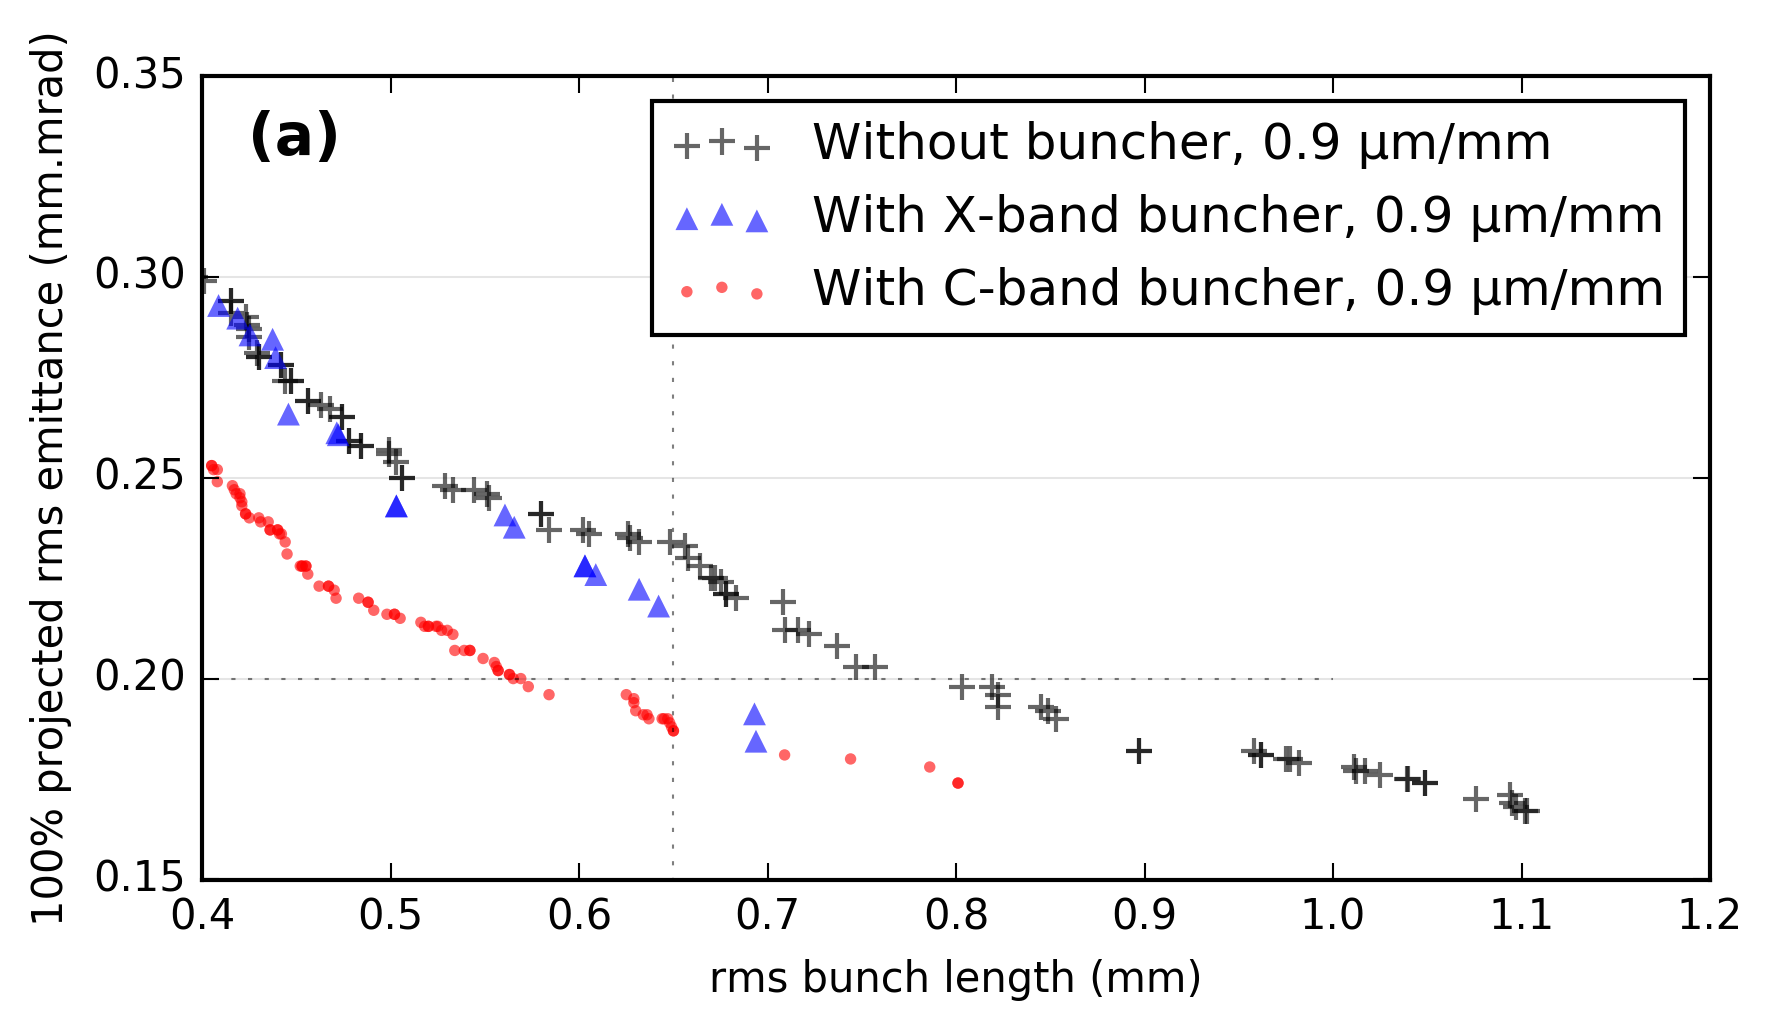
\includegraphics[width=0.6\textwidth]{s120-a}\\
	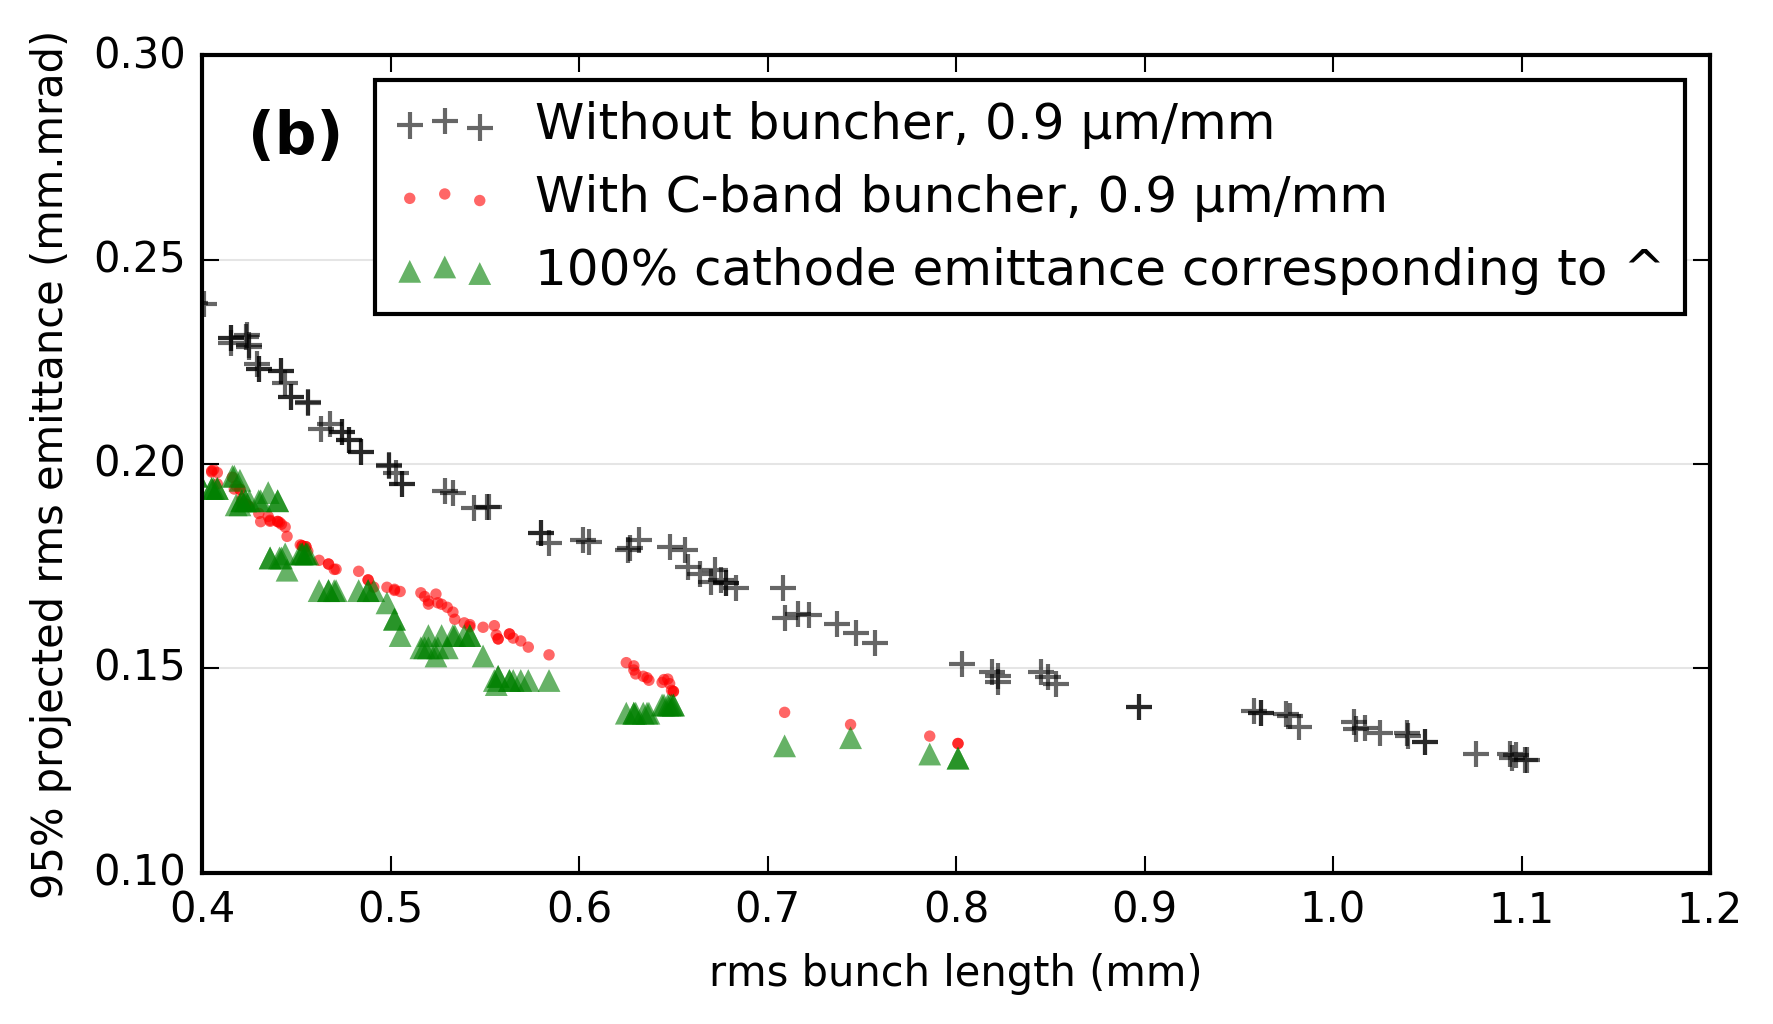
\includegraphics[width=0.6\textwidth]{s120-b}
	\caption{
	200\,pC 束团发射度 vs. rms 长度的一组最优解集。Astra 模拟中采用 10000 宏粒子。图中同时比较了 S 波段光阴极注入器加入 C 波段高频腔与否的发射度优化情形。}
	\label{Pareto120}
\end{figure}

图 \ref{laser_dimension} 是图 \ref{Pareto120} 中给出的优化解集所对应的激光尺寸参数。从图中可以看到,集成了高频腔后,电子枪拥有了在枪的下游对束团进行压缩的能力,从而保持相同的注入器出口峰值流强时,阴极表面的束流峰值流强就可以降低,因此激光纵向可以拉长,由于电荷密度基本不变,其横向尺寸可以缩小,这就减小了阴极上的热发射度。图上对应 \SI{30}{A} 峰值流强的位置,相较于无高频腔的情形其对应激光长度从 \SI{5}{ps} 拉长到了 \SI{10}{ps},而激光半径 $r$ 从 \SI{0.4}{mm} 降低到了 \SI{0.32}{mm}。若此时发射为笔形束的饱和发射情形,则激光长度与 $r^{3/2}$ 成反比,因此当激光长度拉长一倍时,激光半径的减小比例应为 37\%,然而如前所述,遗传算法优化器选择了 20\% 的减小量,这就暗示了引入了聚束腔后,笔形束的饱和发射(此时阴极束流亮度最高)并不是使注入器出口处亮度最高的情形;而对于无聚束腔的注入器优化结果证明阴极束流亮度最高的同时注入器出口处也取到最高亮度。引入聚束腔而导致的阴极束流最高亮度无法保持的现象的原因需要进一步探索。

图 \ref{laser_dimension} 还表明另一个现象:即使引入聚束腔,激光的束长也没有达到优化中设置的上限值 15\,ps。目前怀疑这是由于初始束团过长导致较大 RF 能散在螺线管线圈中的色散效应造成的。具体原因也有待进一步研究。

图 \ref{Pareto120} 中对应 \SI{30}{A} 峰值流强的优化解的切片发射度见图 \ref{slice_emittance}。图中可以看到,在加入一个聚束腔后,除头尾外整个束团的切片发射度较为统一,均在 \SI{0.15}{\mu m} 附近;相对于无聚束腔的情形,切片发射度得到了 25\% 的减小,且各切片的发射度也更加均匀。若设法将热发射度从 \SI{0.9}{\mu m/mm} 降至 \SI{0.5}{\mu m/mm},优化器给出的核心切片发射度可以降至 \SI{0.1}{\mu m}。图中显示无聚束腔情形核心切片发射度均在 \SI{0.2}{\mu m} 以上,这也说明了当前注入器出口处束流发射度最低也只能测到 \SI{0.2}{\mu m} 左右的原因。

\begin{figure}[htbp]
	\centering
	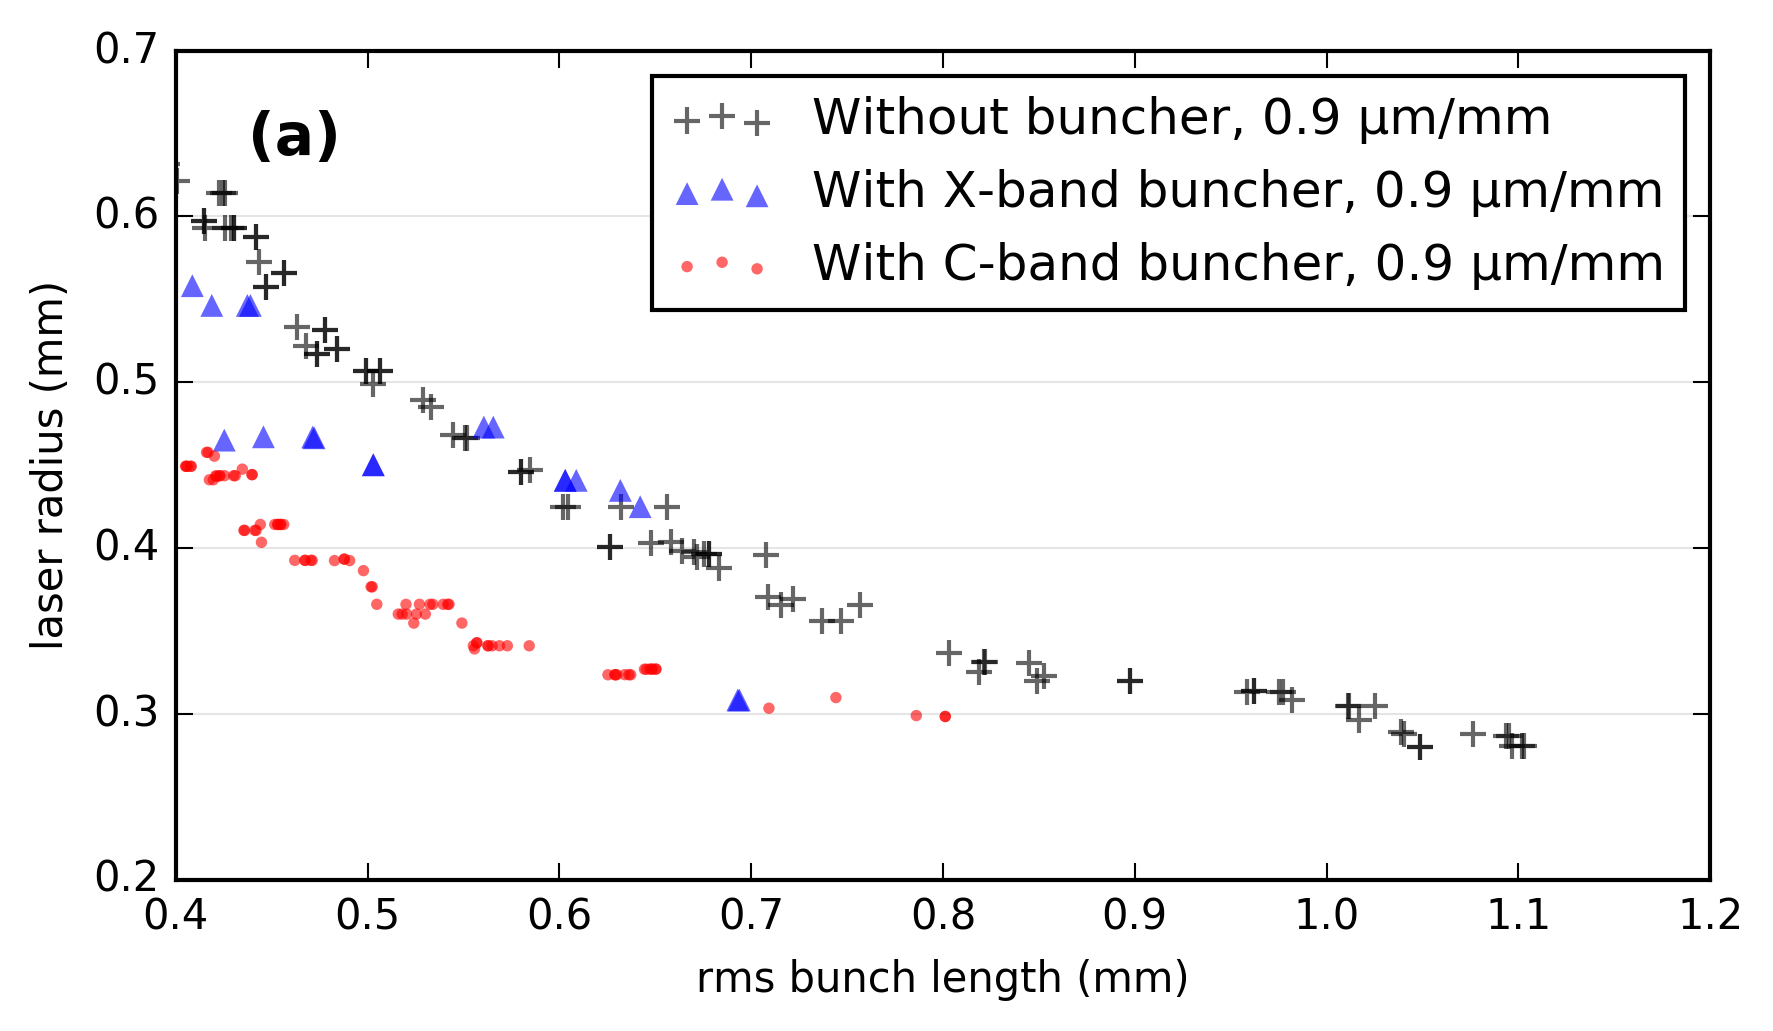
\includegraphics[width=0.6\textwidth]{laser-a}\\
	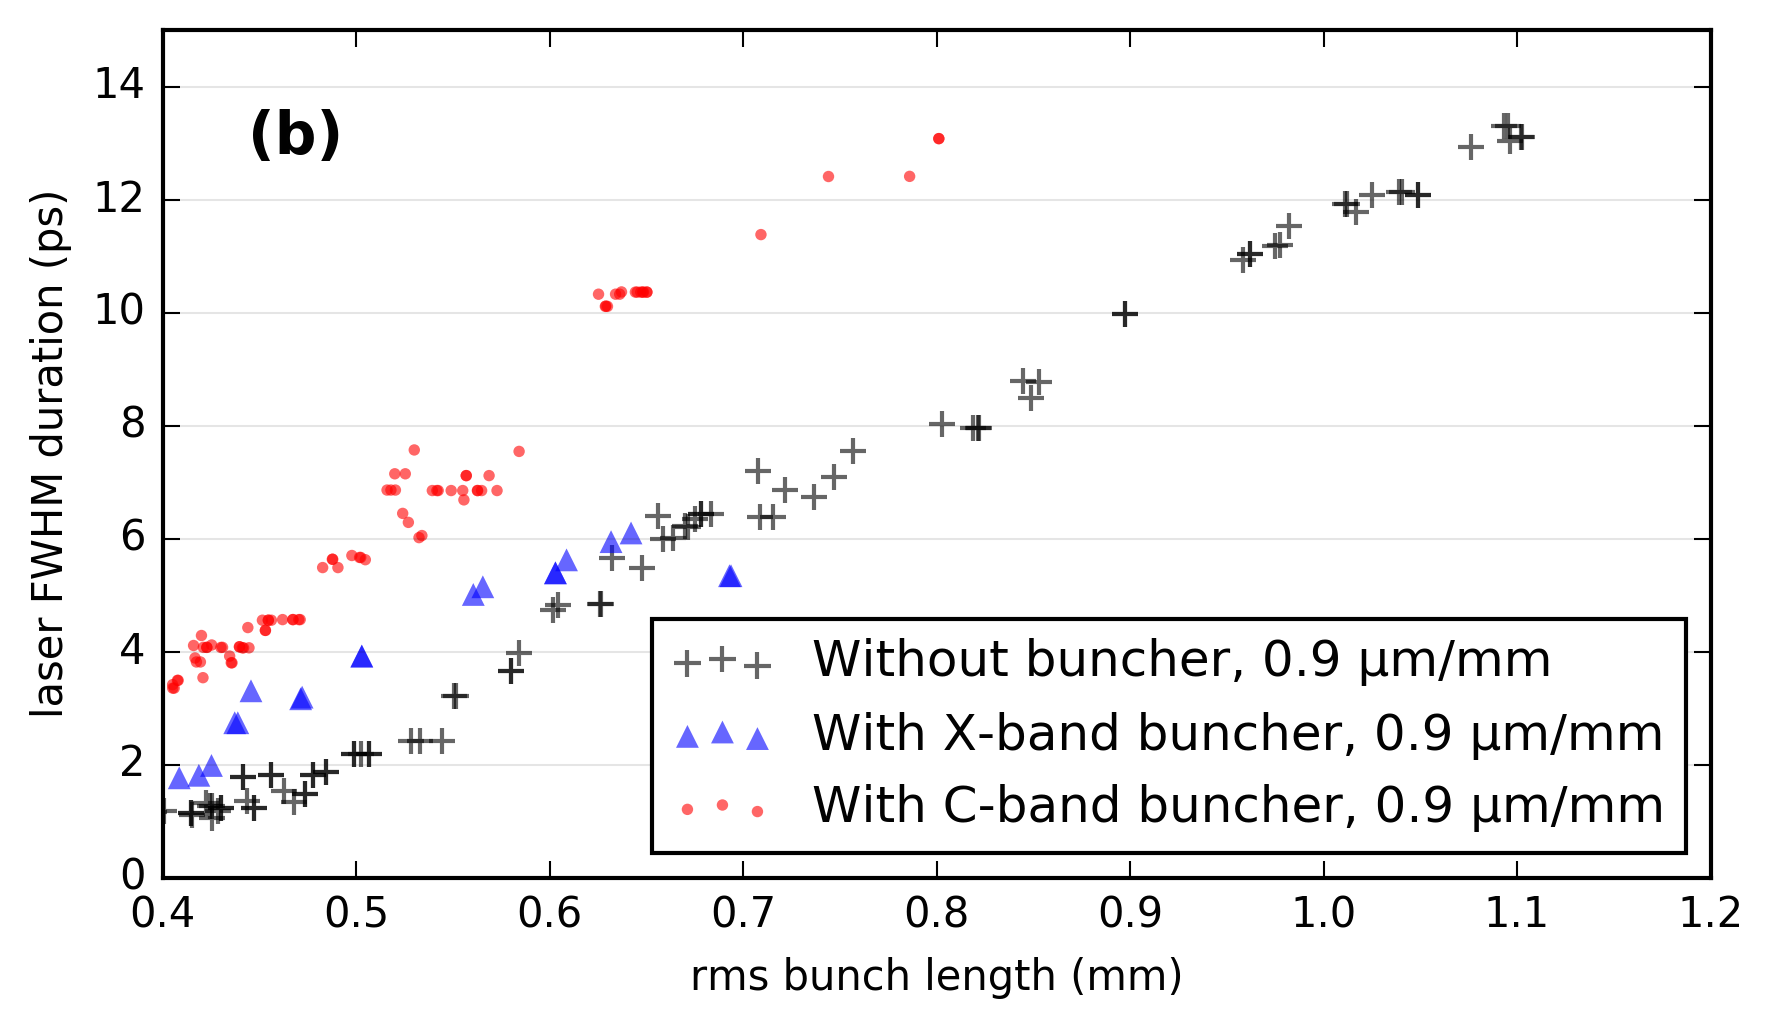
\includegraphics[width=0.6\textwidth]{laser-b}
	\caption{图 \ref{Pareto120} 给出优化结果所对应的激光半径和 FWHM 长度。}
	\label{laser_dimension}
\end{figure}

\begin{figure}[htbp]
	\centering
	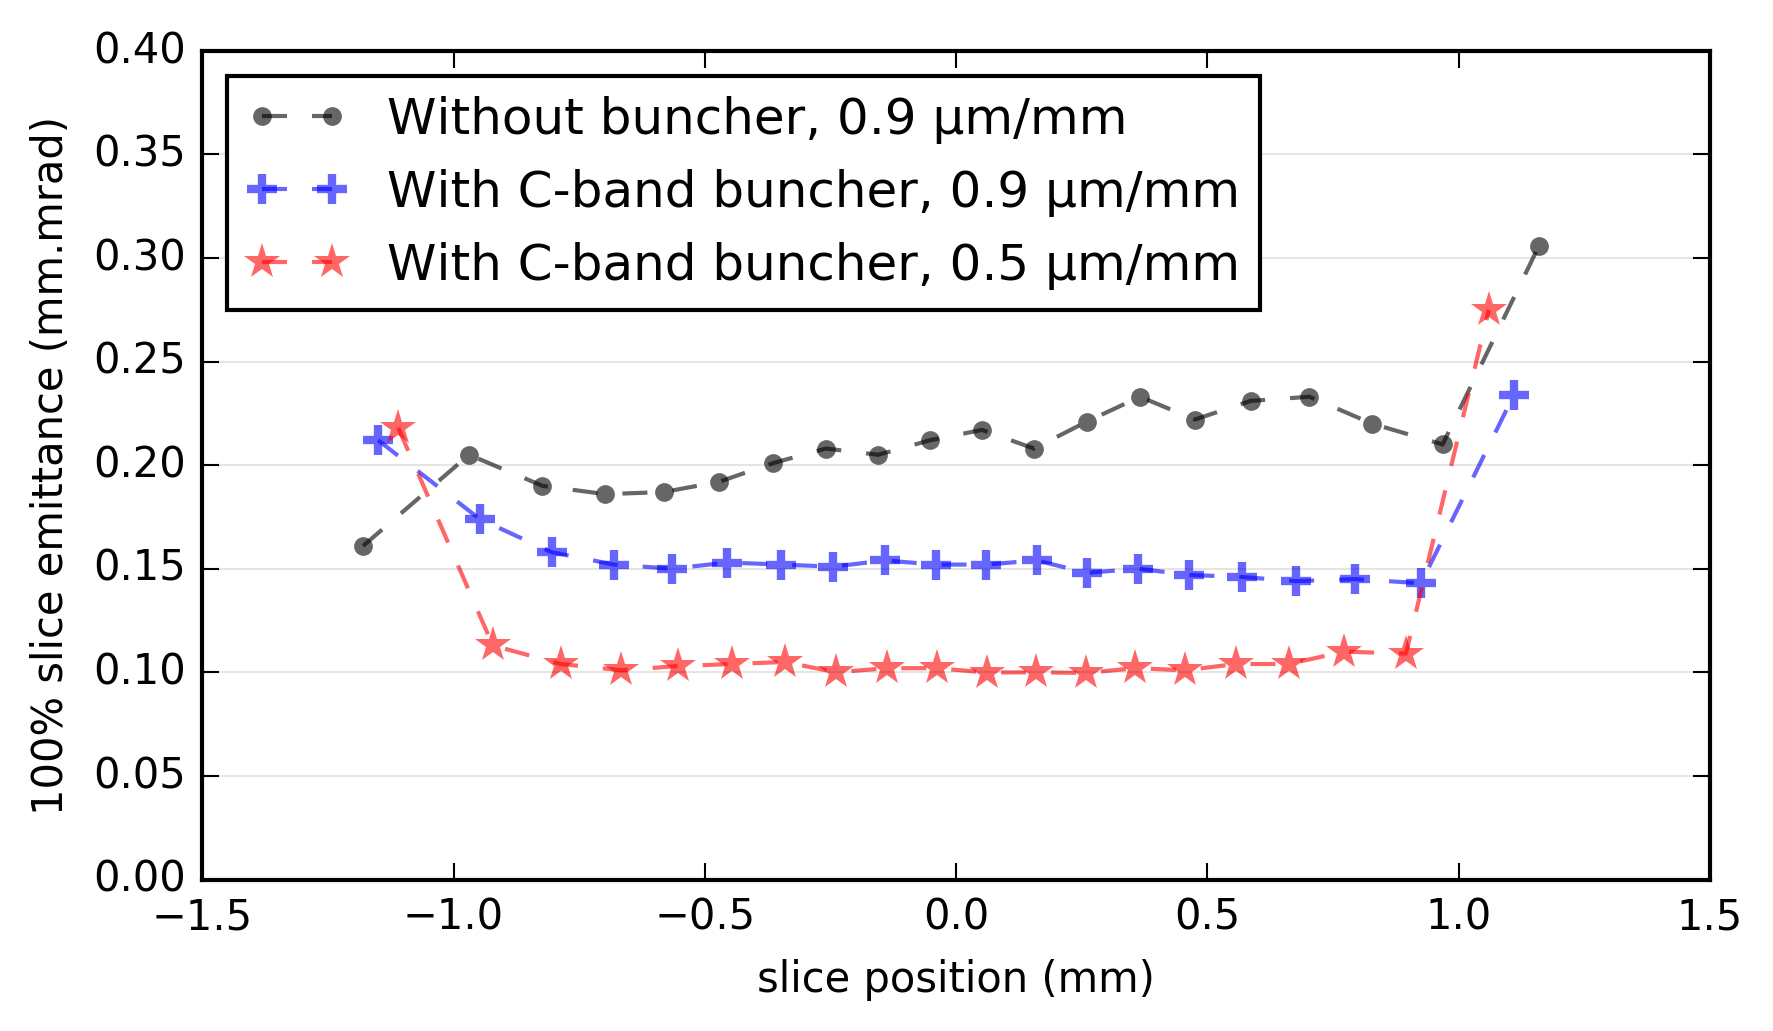
\includegraphics[width=0.6\textwidth]{slice}
	\caption{\SI{200}{pC} 束团,注入器出口处 \SI{30}{A} 峰值流强的优化解的切片发射度。Astra 模拟中采用了 20000 宏粒子。}
	\label{slice_emittance}
\end{figure}

\subsubsection{S/X 合并型双频腔注入器}
我们首先用遗传算法优化器优化了合并型 S/X 双频电子枪注入器,其束线布局见图 \ref{fig:injector-x}。束线包括一个 BNL 型 S 波段电子枪(腔梯度设置为 \SI{120}{MV/m}),一个发射度补偿螺线管线圈,一个 X 波段聚束腔和两节 S 波段行波加速管(每节加速管加速梯度 $<$ \SI{78}{MV})。光阴极上的激光纵向分布为均匀分布,横向分布为在一倍标准差处截断的高斯分布。激光的横向/纵向尺寸,S 波段电子枪相位,X 波段聚束腔梯度及相位,螺线管线圈强度,行波加速管的梯度和位置作为优化器的待优化变量。

图 \ref{Pareto120}(a)比较了 S/X 双频腔注入器、S/C 双频腔注入器与 S 波段电子枪注入器的 Pareto 前沿。从图中可以看到,在 rms 束团长度小于 \SI{0.65}{mm}(峰值流强小于 \SI{30}{A})时,加入 X 波段聚束腔的优化结果趋近于无聚束腔的情形,当 rms 束团长度大于 \SI{0.65}{mm},X 波段聚束腔的优化结果趋向于 C 波段聚束腔的优化结果。分离型和合并型双频电子枪性能的差异有待进一步分析。

\subsubsection{高频腔选取不同波段的优化结果对比}

\subsubsection{分离型和合并型双频电子枪性能差异的分析}

\section{非线性发射区注入器束流亮度的研究}

\section{小结}
本章首先分析了现代注入器中光阴极发射常用的配置:扁平束和笔形束,在阴极上的初始极限热发射度,给出了极限热发射度的公式及达成条件,并从极限热发射度的角度说明笔形束相对于扁平束的优势。随后讨论了光阴极注入器中电子束从产生到传输至注入器出口过程中,对发射度及束流品质可能造成影响的各个因素,由此引出光阴极注入器优化的复杂性:多变量及多优化目标。在明确笔形束可以更好地保持热发射度到注入器出口这一事实后,我们由空间叠加型双频电子枪的思路启发,引入了空间分离型双频光阴极微波电子枪的概念,并设计优化算法对腔型进行了优化。对双频电子枪注入器的动力学进行验证时,由于问题的多变量多优化目标本质,我们开发了基于 NSGA-II 的遗传算法优化器,以清华大学探索 100 高性能计算平台为依托对双频电子枪注入器进行了优化。共采用遗传算法优化了两种配置的注入器,即合并型 S/X 双频电子枪注入器和分离型 S/C 双频电子枪注入器。遗传算法优化结果表面,加入一个高频腔可以将注入器出口处 \SI{200}{pC},峰值流强 \SI{30}{A} 的束流的发射度降低 $\sim$ 25\%,且切片发射度近乎与热发射度相等,意味着双频电子枪能够将束流的初始横向亮度保持到注入器出口处。当设法将归一化热发射度降低至 \SI{0.5}{\mu m/mm} 时,优化得到了注入器出口处流强 \SI{30}{A} 时切片发射度 $\sim$ \emit{0.10} 的注入器方案。然而双频电子枪注入器遗传算法优化中依然有一些未解决的问题,例如优化器并没有在高频腔存在时充分利用其可以对束流进行聚束的能力,初始束团并没有取到预期的长度(例如 \SI{20}{ps});以及在高频腔存在时,注入器出口处优化解并不是空间电荷限发射情形,也即束流没有取到极限热发射度。以上问题的产生原因有待进一步理论及模拟探究。
